\documentclass{report}
\usepackage[usenames]{color}
\usepackage[english]{babel}
\usepackage[utf8]{inputenc}
\usepackage{times}
\usepackage{mathptmx}
\usepackage[left=1.5cm,right=6cm,top=1.5cm,bottom=3cm]{geometry}
\usepackage{hyperref}
\usepackage[T1]{fontenc}
\usepackage{tikz}
\usepackage{yfonts}
\usepackage{colortbl}
\usepackage{graphicx}
%\usepackage{translator} % comment this, if not available

\usepackage{listings}
\lstset{language=Python}

\newenvironment{changemargin}[2]{\begin{list}{}{%
\setlength{\topsep}{0pt}%
\setlength{\leftmargin}{0pt}%
\setlength{\rightmargin}{0pt}%
\setlength{\listparindent}{\parindent}%
\setlength{\itemindent}{\parindent}%
\setlength{\parsep}{0pt plus 1pt}%
\addtolength{\leftmargin}{#1}%
\addtolength{\rightmargin}{#2}%
\addtolength{\textwidth}{0 pt minus #1}%
\addtolength{\textwidth}{#2}%
}\item }{\end{list}}
%cmtt
%hlst
%hlh 
%\newcommand\Nmff{augie}
\newcommand\Nmff{iwona} 
%\newcommand\Nmff{kurier}
%\newcommand\Nmff{pzc}   
%\newcommand\Nmff{pag}   
%\newcommand\Nmff{ccr}   
%\newcommand\Nmff{cmss}  
%\newcommand\Nmff{bch}   
%\newcommand\Nmff{fvs}   


\newcommand\Nmfont{\usefont{T1}{\Nmff}{m}{n}\selectfont}
\newcommand\Nmfontb{\usefont{T1}{\Nmff}{m}{sc}\selectfont}
\newcommand\Nm[1]{{\Nmfont{\Nmfontb{#1}}}\index[author]{#1@{#1}}}
\newcommand\XNm[2]{{\Nmfont{#1\nobreak\ {\Nmfontb{#2}}}}\index[author]{#2@{#2 #1}}}
\newcommand\BNm[1]{{\Nmfont\bf {\Nmfontb{#1}}}\index[author]{#1@{#1}}}             
\newcommand\BXNm[2]{{\Nmfont\bf {#1\nobreak\ {\Nmfontb{#2}}}}\index[author]{#2@{#2 #1}}}
\newcommand\NNm[1]{{\Nmfont{\Nmfontb{#1}}}}                                             
\newcommand\NXNm[2]{{\Nmfont{#1\nobreak\ {\Nmfontb{#2}}}}}                              
\newcommand\BNNm[1]{{\Nmfont\bf {\Nmfontb{#1}}}}                                        
\newcommand\BNXNm[2]{{\Nmfont\bf{#1\nobreak\ {\Nmfontb{#2}}}}}                          
\newcommand\Xtitre[1]{\underline{#1}}                                                   
%\usepackage{lineno}
%\runninglinenumbers
%\modulolinenumbers[5]



\makeatletter                    
\definecolor{bl}{rgb}{0,0.2,0.6} 
\let\LaTeX@startsection\@startsection
\renewcommand{\@startsection}[6]{\LaTeX@startsection%
{#1}{#2}{#3}{#4}{#5}{\color{bl}\raggedright #6}}     
\makeatother                                   

\title{Python Computer Vision Framework}
\author{Bertrand NOUVEL}
\date{\includegraphics[width=6cm]{pycvf.png}\\2009\\ Development Release\\ \vspace{2cm} \\
\includegraphics[width=6cm]{logo_jfli.png}}


\begin{document}

\maketitle
\tableofcontents

\chapter{Forewords}
\section{This is a development version}
The API is described here in order to help people to start using better framework than previous ones.

However, the project has grown very quickly, and some part of the design of the software has still to be rethought to be more clear.
Thus, be aware that the elements you will find in this documentation are likely to change (for better) within one year.






!!!Not yet finished!!!




\section{What's wrong with previous Frameworks ?}
\subsection{Which Frameworks ??}
A Framework is not a toolkit. A library offers you facility to access a resource. A toolkit guide you in the way
of writing application using that toolkit. A Framework drives you even more, in order to make upcoming applications also part of 
the framework.

So there is the question of which Framework.Althought to do computer vision
is supposed to be cool and popular, there is not that much good integrated software framework.
Supposedly the community is addicted to Matlab, but I know some of us refused this choice,
and stayed for a longtime on C and C++.





\section{Why to do a Python Framework ?}
\subsection{Well programmed Python can be REALLY FAST !}
One of the factor that have made Computer Vision stucked to {\tt C} and {\tt C++} programming is the fact they were affraid of loosing performance in switching to a higher level language.
It is true that if all the access to individual cell of the pixels of a video array have to be interpreted and checked over bounds, range and so on, your program may easily run 1000 slower 
then its C version.





\subsection{Python allow OBJECTS and LAMBDAs !}
One of the complication of C++, it that everything is typed, you cannot easily add or remove parameters to functions, 
moreover a function which take has a argument a function, takes only the function pointer as argument, 
and the context in which it execute has to be a second argument of the function.
This generally make these kind of function quite specific, or messy and untyped.

In python you can easily create things like that would be complicated to implement else :





\begin{minipage}{\textwidth}
{\small
% Generator: GNU source-highlight, by Lorenzo Bettini, http://www.gnu.org/software/src-highlite
\noindent
\mbox{}l=\textbf{range}(10) \\
\mbox{}\textbf{class}\ Fib: \\
\mbox{}\ \ \textbf{def}\ \textbf{$\_$$\_$init$\_$$\_$}(self): \\
\mbox{}\ \ \ \ \ self.value=0 \\
\mbox{}\ \ \textbf{def}\ \textbf{method}(self,v): \\
\mbox{}\ \ \ \ \ self.value+=v \\
\mbox{} \\
\mbox{}fib=\textbf{Fib}() \\
\mbox{}\textbf{map}(fib.method,l) \\
\mbox{}\textit{\#\#$>$$>$\ [None,\ None,\ None,\ None,\ None,\ None,\ None,\ None,\ None,\ None]} \\
\mbox{}\textit{\#\#$>$$>$\ } \\
\mbox{}\textit{\#\#$>$$>$\ } \\
\mbox{} \\
\mbox{}\textbf{print}\ fib.value \\
\mbox{}\textit{\#\#$>$$>$\ 45} \\
\mbox{}\textit{\#\#$>$$>$\ } \\
\mbox{}\textit{\#\#$>$$>$\ } \\
\mbox{} \\
\mbox{}
}
\end{minipage}





\subsection{Python is FREE !}
 Matlab has the big inconvenient of not being a free software. Of course, they exists free alternative as octave.
 But Matlab remains the reference.






\subsection{Python community is ALIVE !}
The number of open-source project in Python is turnint to be more than "5%"










Python programmers code more efficiently since, although having many program in python, 
they they have less line to change thant their challengers.






Also, there is much more "Python" Programmers thant Matlab programmers.
Actually, Matlab has never emerged as a good language for writing complex applications.














\chapter{Installation of the Framework}
The framework so far has been developped and used under "Linux Ubuntu 8.04/9.04"


However, it should be easily portable to other systems.


It is not yet for diffusion, and is planed to remain closed source for a while.
We plan tor progressively make it opensource are the user number will increase.



The environement provides you access to all the necessaries binary packages.
Congratulations. You are now ready to use the framework.




\section{Installation on your machine with Ubuntu Linux}
The framework requires quite a lot of software to work properly.

This section is to be updated with help of the users...










\lstset{
language=bash,                % choose the language of the code
basicstyle=\footnotesize,       % the size of the fonts that are used for the code
numbers=left,                   % where to put the line-numbers
numberstyle=\footnotesize,      % the size of the fonts that are used for the line-numbers
stepnumber=5,                   % the step between two line-numbers. If it's 1 each line will be numbered
numbersep=5pt,                  % how far the line-numbers are from the code
backgroundcolor=\color{white},  % choose the background color. You must add \usepackage{color}
showspaces=false,               % show spaces adding particular underscores
showstringspaces=false,         % underline spaces within strings
showtabs=false,                 % show tabs within strings adding particular underscores
frame=single,	                % adds a frame around the code
tabsize=2,	                % sets default tabsize to 2 spaces
captionpos=b,                   % sets the caption-position to bottom
breaklines=true,                % sets automatic line breaking
breakatwhitespace=false         % sets if automatic breaks should only happen at whitespace
}
\begin{lstlisting}
sudo apt-get install python2.6-minimal python-yahoo python-support python-sphinx python-simplejson \
  python-sip4 python-sip4-dev python-scientific python-reportlab python-qt4 python-qt4-gl python-qt4-dbus \
  python-pywt python-pycurl python-ao python-numpy python-matplotlib python-matplotlib-data python-kde4 \
  python-kde4-dev python-feedparser python-dev python-beautifulsoup

\end{lstlisting}







\section{Generic Installation from the source}
The framework requires quite a lot of software to work properly.

Here is a list of required softwares

 Python 2.6 
 BeautifulSoup 
 ctype 
 Cython  
 cmake 
 gccxml   
 numpy( implies lapack, clapack, blas, atlas, fftw) 
 scipy 
 matplotlib ( implies freetype)
 Imaging 
 OpenCv 
 FFMPEG 
 PyFFMPEG 
 Orange 
 Shogun 
 PyQt4 (implies Sip) 
 (optionally ) PyKDE4 (which implies fontconfig, automoc, soprano, strigi, kdelibs, kdebase , kdebase-runtime, pykde4)


This section is to be updated with help of the users...















\chapter{Essentials of Python for Scientists}
There exists already numerous tutorials on the topic, that cover in-depth many aspects of python in Science.

*  The python tutorial.

*  The numpy tutorial.
*  The very good numpy for matlab users.

* The scipy course online.



\section{Numeric Python}
\lstset{
language=Python,                % choose the language of the code
basicstyle=\footnotesize,       % the size of the fonts that are used for the code
numbers=left,                   % where to put the line-numbers
numberstyle=\footnotesize,      % the size of the fonts that are used for the line-numbers
stepnumber=5,                   % the step between two line-numbers. If it's 1 each line will be numbered
numbersep=5pt,                  % how far the line-numbers are from the code
backgroundcolor=\color{white},  % choose the background color. You must add \usepackage{color}
showspaces=false,               % show spaces adding particular underscores
showstringspaces=false,         % underline spaces within strings
showtabs=false,                 % show tabs within strings adding particular underscores
frame=single,	                % adds a frame around the code
tabsize=2,	                % sets default tabsize to 2 spaces
captionpos=b,                   % sets the caption-position to bottom
breaklines=true,                % sets automatic line breaking
breakatwhitespace=false         % sets if automatic breaks should only happen at whitespace
}
\begin{lstlisting}
import numpy

\end{lstlisting}















\begin{minipage}{\textwidth}
{\small
% Generator: GNU source-highlight, by Lorenzo Bettini, http://www.gnu.org/software/src-highlite
\noindent
\mbox{}\textbf{import}\ numpy \\
\mbox{} \\
\mbox{}z=numpy.\textbf{zeros}((2,2,2)) \\
\mbox{}\textbf{print}\ z \\
\mbox{}\textit{\#\#$>$$>$\ [[[\ 0.\ \ 0.]} \\
\mbox{}\textit{\#\#$>$$>$\ \ \ [\ 0.\ \ 0.]]} \\
\mbox{}\textit{\#\#$>$$>$\ } \\
\mbox{}\textit{\#\#$>$$>$\ \ [[\ 0.\ \ 0.]} \\
\mbox{}\textit{\#\#$>$$>$\ \ \ [\ 0.\ \ 0.]]]} \\
\mbox{}\textit{\#\#$>$$>$\ } \\
\mbox{}\textit{\#\#$>$$>$\ } \\
\mbox{} \\
\mbox{}o=numpy.\textbf{ones}((2,2)) \\
\mbox{}\textbf{print}\ o \\
\mbox{}\textit{\#\#$>$$>$\ [[\ 1.\ \ 1.]} \\
\mbox{}\textit{\#\#$>$$>$\ \ [\ 1.\ \ 1.]]} \\
\mbox{}\textit{\#\#$>$$>$\ } \\
\mbox{}\textit{\#\#$>$$>$\ } \\
\mbox{} \\
\mbox{}e=numpy.\textbf{eye}(2) \\
\mbox{}e \\
\mbox{}\textit{\#\#$>$$>$\ array([[\ 1.,\ \ 0.],} \\
\mbox{}\textit{\#\#$>$$>$\ \ \ \ \ \ \ \ [\ 0.,\ \ 1.]])} \\
\mbox{}\textit{\#\#$>$$>$\ } \\
\mbox{}\textit{\#\#$>$$>$\ } \\
\mbox{} \\
\mbox{}r=numpy.random.\textbf{random}((3,3)) \\
\mbox{} \\
\mbox{}
}
\end{minipage}





\section{Scientific Python}
\lstset{
language=Python,                % choose the language of the code
basicstyle=\footnotesize,       % the size of the fonts that are used for the code
numbers=left,                   % where to put the line-numbers
numberstyle=\footnotesize,      % the size of the fonts that are used for the line-numbers
stepnumber=5,                   % the step between two line-numbers. If it's 1 each line will be numbered
numbersep=5pt,                  % how far the line-numbers are from the code
backgroundcolor=\color{white},  % choose the background color. You must add \usepackage{color}
showspaces=false,               % show spaces adding particular underscores
showstringspaces=false,         % underline spaces within strings
showtabs=false,                 % show tabs within strings adding particular underscores
frame=single,	                % adds a frame around the code
tabsize=2,	                % sets default tabsize to 2 spaces
captionpos=b,                   % sets the caption-position to bottom
breaklines=true,                % sets automatic line breaking
breakatwhitespace=false         % sets if automatic breaks should only happen at whitespace
}
\begin{lstlisting}
pyplot.clf()
pyplot.gray()
pyplot.imshow(scipy.lena())

pyplot.show()

\end{lstlisting}















\noindent
\includegraphics[width=\textwidth]{pyfig-ab2809c07efd01ed3d924a69f951aa28.pdf}








\lstset{
language=Python,                % choose the language of the code
basicstyle=\footnotesize,       % the size of the fonts that are used for the code
numbers=left,                   % where to put the line-numbers
numberstyle=\footnotesize,      % the size of the fonts that are used for the line-numbers
stepnumber=5,                   % the step between two line-numbers. If it's 1 each line will be numbered
numbersep=5pt,                  % how far the line-numbers are from the code
backgroundcolor=\color{white},  % choose the background color. You must add \usepackage{color}
showspaces=false,               % show spaces adding particular underscores
showstringspaces=false,         % underline spaces within strings
showtabs=false,                 % show tabs within strings adding particular underscores
frame=single,	                % adds a frame around the code
tabsize=2,	                % sets default tabsize to 2 spaces
captionpos=b,                   % sets the caption-position to bottom
breaklines=true,                % sets automatic line breaking
breakatwhitespace=false         % sets if automatic breaks should only happen at whitespace
}
\begin{lstlisting}
import scipy

l=scipy.lena()
scipy.fft2(l)

\end{lstlisting}

















\lstset{
language=Python,                % choose the language of the code
basicstyle=\footnotesize,       % the size of the fonts that are used for the code
numbers=left,                   % where to put the line-numbers
numberstyle=\footnotesize,      % the size of the fonts that are used for the line-numbers
stepnumber=5,                   % the step between two line-numbers. If it's 1 each line will be numbered
numbersep=5pt,                  % how far the line-numbers are from the code
backgroundcolor=\color{white},  % choose the background color. You must add \usepackage{color}
showspaces=false,               % show spaces adding particular underscores
showstringspaces=false,         % underline spaces within strings
showtabs=false,                 % show tabs within strings adding particular underscores
frame=single,	                % adds a frame around the code
tabsize=2,	                % sets default tabsize to 2 spaces
captionpos=b,                   % sets the caption-position to bottom
breaklines=true,                % sets automatic line breaking
breakatwhitespace=false         % sets if automatic breaks should only happen at whitespace
}
\begin{lstlisting}
l=scipy.lena()
# compute FFT
r=numpy.log(1+numpy.abs(numpy.fft.fft2(l)))
# recenter FFT so it displays nicely
r=numpy.roll(r,r.shape[0]//2,axis=0)
r=numpy.roll(r,r.shape[1]//2,axis=1)

pyplot.clf();pyplot.jet();pyplot.colorbar();pyplot.imshow(r)

pyplot.show()

\end{lstlisting}















\noindent
\includegraphics[width=\textwidth]{pyfig-ea3a0e4746cc8d7e0092a4516bdb92b4.pdf}










\lstset{
language=Python,                % choose the language of the code
basicstyle=\footnotesize,       % the size of the fonts that are used for the code
numbers=left,                   % where to put the line-numbers
numberstyle=\footnotesize,      % the size of the fonts that are used for the line-numbers
stepnumber=5,                   % the step between two line-numbers. If it's 1 each line will be numbered
numbersep=5pt,                  % how far the line-numbers are from the code
backgroundcolor=\color{white},  % choose the background color. You must add \usepackage{color}
showspaces=false,               % show spaces adding particular underscores
showstringspaces=false,         % underline spaces within strings
showtabs=false,                 % show tabs within strings adding particular underscores
frame=single,	                % adds a frame around the code
tabsize=2,	                % sets default tabsize to 2 spaces
captionpos=b,                   % sets the caption-position to bottom
breaklines=true,                % sets automatic line breaking
breakatwhitespace=false         % sets if automatic breaks should only happen at whitespace
}
\begin{lstlisting}
def powerspectrum_only(i):
  return numpy.real(numpy.fft.ifft2(abs(numpy.fft.fft2(i))))

r=powerspectrum_only(scipy.lena())

pyplot.clf();pyplot.jet();pyplot.colorbar();pyplot.imshow(r)

pyplot.show()

\end{lstlisting}















\noindent
\includegraphics[width=\textwidth]{pyfig-57a80b38750b3fdf8a224dd607ad2e46.pdf}











\lstset{
language=Python,                % choose the language of the code
basicstyle=\footnotesize,       % the size of the fonts that are used for the code
numbers=left,                   % where to put the line-numbers
numberstyle=\footnotesize,      % the size of the fonts that are used for the line-numbers
stepnumber=5,                   % the step between two line-numbers. If it's 1 each line will be numbered
numbersep=5pt,                  % how far the line-numbers are from the code
backgroundcolor=\color{white},  % choose the background color. You must add \usepackage{color}
showspaces=false,               % show spaces adding particular underscores
showstringspaces=false,         % underline spaces within strings
showtabs=false,                 % show tabs within strings adding particular underscores
frame=single,	                % adds a frame around the code
tabsize=2,	                % sets default tabsize to 2 spaces
captionpos=b,                   % sets the caption-position to bottom
breaklines=true,                % sets automatic line breaking
breakatwhitespace=false         % sets if automatic breaks should only happen at whitespace
}
\begin{lstlisting}
def phase_only(i):
  return numpy.real(numpy.fft.ifft2(numpy.exp(1J*scipy.angle(numpy.fft.fft2(i)))))

r=phase_only(scipy.lena())

pyplot.clf();pyplot.jet();pyplot.colorbar();pyplot.imshow(r)

pyplot.show()

\end{lstlisting}















\noindent
\includegraphics[width=\textwidth]{pyfig-9fdcc79eabdaced297af4fd09aa29aee.pdf}



















\section{PyFFMPEG 2 alpha Essentials}
\subsection{Playing VideoFiles}
\lstset{
language=bash,                % choose the language of the code
basicstyle=\footnotesize,       % the size of the fonts that are used for the code
numbers=left,                   % where to put the line-numbers
numberstyle=\footnotesize,      % the size of the fonts that are used for the line-numbers
stepnumber=5,                   % the step between two line-numbers. If it's 1 each line will be numbered
numbersep=5pt,                  % how far the line-numbers are from the code
backgroundcolor=\color{white},  % choose the background color. You must add \usepackage{color}
showspaces=false,               % show spaces adding particular underscores
showstringspaces=false,         % underline spaces within strings
showtabs=false,                 % show tabs within strings adding particular underscores
frame=single,	                % adds a frame around the code
tabsize=2,	                % sets default tabsize to 2 spaces
captionpos=b,                   % sets the caption-position to bottom
breaklines=true,                % sets automatic line breaking
breakatwhitespace=false         % sets if automatic breaks should only happen at whitespace
}
\begin{lstlisting}
cd pyffmpeg2-alpha-candidate
cd examples
python playvideo_qt_alsa.py videofile.mpg

\end{lstlisting}






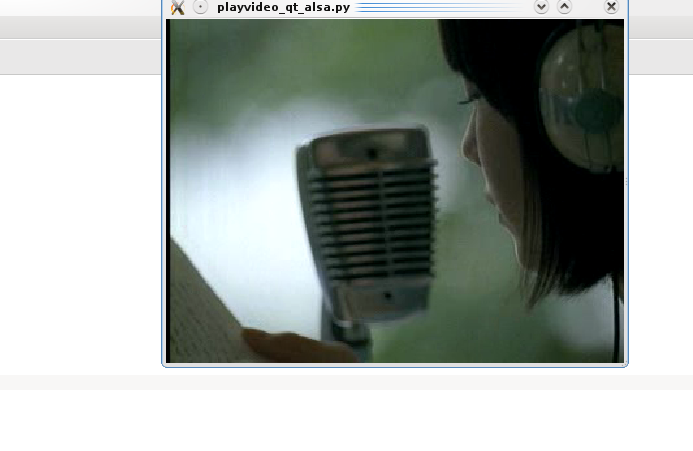
\includegraphics[width=5cm]{playvideoqt.png}






\subsection{Loading VideoFiles}
\lstset{
language=Python,                % choose the language of the code
basicstyle=\footnotesize,       % the size of the fonts that are used for the code
numbers=left,                   % where to put the line-numbers
numberstyle=\footnotesize,      % the size of the fonts that are used for the line-numbers
stepnumber=5,                   % the step between two line-numbers. If it's 1 each line will be numbered
numbersep=5pt,                  % how far the line-numbers are from the code
backgroundcolor=\color{white},  % choose the background color. You must add \usepackage{color}
showspaces=false,               % show spaces adding particular underscores
showstringspaces=false,         % underline spaces within strings
showtabs=false,                 % show tabs within strings adding particular underscores
frame=single,	                % adds a frame around the code
tabsize=2,	                % sets default tabsize to 2 spaces
captionpos=b,                   % sets the caption-position to bottom
breaklines=true,                % sets automatic line breaking
breakatwhitespace=false         % sets if automatic breaks should only happen at whitespace
}
\begin{lstlisting}
# basic code for playing a movie (but that so far actually does not display anything)
from pyffmpegb import FFMpegReader
p=FFMpegReader()
mp.open(sys.argv[1])
mp.run()

\end{lstlisting}











It is now time to actually do something, let's try to compute the luminance of each frame and to display it on the console :





\lstset{
language=Python,                % choose the language of the code
basicstyle=\footnotesize,       % the size of the fonts that are used for the code
numbers=left,                   % where to put the line-numbers
numberstyle=\footnotesize,      % the size of the fonts that are used for the line-numbers
stepnumber=5,                   % the step between two line-numbers. If it's 1 each line will be numbered
numbersep=5pt,                  % how far the line-numbers are from the code
backgroundcolor=\color{white},  % choose the background color. You must add \usepackage{color}
showspaces=false,               % show spaces adding particular underscores
showstringspaces=false,         % underline spaces within strings
showtabs=false,                 % show tabs within strings adding particular underscores
frame=single,	                % adds a frame around the code
tabsize=2,	                % sets default tabsize to 2 spaces
captionpos=b,                   % sets the caption-position to bottom
breaklines=true,                % sets automatic line breaking
breakatwhitespace=false         % sets if automatic breaks should only happen at whitespace
}
\begin{lstlisting}
from pyffmpegb import FFMpegReader

p=FFMpegReader()

mp.open(sys.argv[1])
tracks=mp.get_tracks()

def event_processor(video_packet):
  video_image,video_time_code = video_packet
  print video_time_code, video_image.shape, video_image.mean()

tracks[0].set_observer(event_processor)
mp.run()

\end{lstlisting}











The open function can actually take a very important parameter called the track\_selector.
Using this parameter you may define which track\footnote{also called ``streams''} from the file you want to open,  how you want to open each track.

Here are some examples of track selectors:





\lstset{
language=Python,                % choose the language of the code
basicstyle=\footnotesize,       % the size of the fonts that are used for the code
numbers=left,                   % where to put the line-numbers
numberstyle=\footnotesize,      % the size of the fonts that are used for the line-numbers
stepnumber=5,                   % the step between two line-numbers. If it's 1 each line will be numbered
numbersep=5pt,                  % how far the line-numbers are from the code
backgroundcolor=\color{white},  % choose the background color. You must add \usepackage{color}
showspaces=false,               % show spaces adding particular underscores
showstringspaces=false,         % underline spaces within strings
showtabs=false,                 % show tabs within strings adding particular underscores
frame=single,	                % adds a frame around the code
tabsize=2,	                % sets default tabsize to 2 spaces
captionpos=b,                   % sets the caption-position to bottom
breaklines=true,                % sets automatic line breaking
breakatwhitespace=false         % sets if automatic breaks should only happen at whitespace
}
\begin{lstlisting}
TS_VIDEO_RGB24={ 'video1':(0, -1, {'pixel_format':PixelFormats.RGB24}), 'audio1':(1,-1,{})}
TS_VIDEO_BGR24={ 'video1':(0, -1, {'pixel_format':PixelFormats.BGR24}), 'audio1':(1,-1,{})}
TS_VIDEO_GRAY8={ 'video1':(0, -1, {'pixel_format':PixelFormats.GRAY8,'videoframebanksz':1, 'skip_frame':32})}

\end{lstlisting}












As you can see track selectors are disctionaries whose value are triplets.
The first element of the triplet, which can be 0 or 1 define the nature of the track, 'video' or 'audio'. 
The second element of the triplet, define the stream number in the file, negative number indicate to query only "compatible streams". Thus -1 generally denotes the default track of the speciefied type.
The third argument is a dictionary of options to be passed to the decoder. The options are of course dependant on the decoder being used.

For video tracks you may set the following option, a pixel_format, the size of the frame buffer (this buffer is normally useless, but I had some problem with some files where frame where still interleaved, 
and I prefer to keep it to face possible buggy decoders), the skip_frame argument may be used to specified whether all frames should be read, or whether we should only read key_frames. You can get more information
on this field py reading related ffmpeg header files. There is also option for rescaling the output.







\subsection{Extracting Keyframes}
\lstset{
language=Python,                % choose the language of the code
basicstyle=\footnotesize,       % the size of the fonts that are used for the code
numbers=left,                   % where to put the line-numbers
numberstyle=\footnotesize,      % the size of the fonts that are used for the line-numbers
stepnumber=5,                   % the step between two line-numbers. If it's 1 each line will be numbered
numbersep=5pt,                  % how far the line-numbers are from the code
backgroundcolor=\color{white},  % choose the background color. You must add \usepackage{color}
showspaces=false,               % show spaces adding particular underscores
showstringspaces=false,         % underline spaces within strings
showtabs=false,                 % show tabs within strings adding particular underscores
frame=single,	                % adds a frame around the code
tabsize=2,	                % sets default tabsize to 2 spaces
captionpos=b,                   % sets the caption-position to bottom
breaklines=true,                % sets automatic line breaking
breakatwhitespace=false         % sets if automatic breaks should only happen at whitespace
}
\begin{lstlisting}
# basic code for playing a movie (but that so far actually does not display anything)
p=FFMpegReader()
TS_VIDEO_GRAY8={ 'video1':(0, -1, {'pixel_format':PixelFormats.GRAY8,'videoframebanksz':1, 'skip_frame':32})}
mp.open(sys.argv[1],TS_VIDEO_GRAY8)

def event_processor(video_packet):
  video_image,video_time_code = video_packet
  print video_time_code, video_image.shape, video_image.mean()

mp.run()

\end{lstlisting}






\subsection{Checking parameters of file}
\begin{minipage}{\textwidth}
{\small
% Generator: GNU source-highlight, by Lorenzo Bettini, http://www.gnu.org/software/src-highlite
\noindent
\mbox{}\textbf{from}\ pyffmpegb\ \textbf{import}\ * \\
\mbox{}mp=\textbf{FFMpegReader}() \\
\mbox{}TS$\_$VIDEO$\_$GRAY8=\{\ \texttt{'video1'}:(0,\ -1,\ \{\texttt{'pixel$\_$format'}:PixelFormats.GRAY8,\texttt{'videoframebanksz'}:1,\ \texttt{'skip$\_$frame'}:32\})\} \\
\mbox{}mp.\textbf{open}(\texttt{"{}/home/tranx/conan1.flv"{}},TS$\_$VIDEO$\_$GRAY8) \\
\mbox{}t=mp.\textbf{get$\_$tracks}() \\
\mbox{}t[0].\textbf{get$\_$fps}() \\
\mbox{}\textit{\#\#$>$$>$\ 29.970029830932617} \\
\mbox{}\textit{\#\#$>$$>$\ } \\
\mbox{}\textit{\#\#$>$$>$\ } \\
\mbox{}mp.\textbf{duration}() \\
\mbox{}\textit{\#\#$>$$>$\ 494681000L} \\
\mbox{}\textit{\#\#$>$$>$\ } \\
\mbox{}\textit{\#\#$>$$>$\ } \\
\mbox{}mp.\textbf{step}() \\
\mbox{}mp.\textbf{get$\_$current$\_$frame}()[0][0] \\
\mbox{}\textit{\#\#$>$$>$\ 2603000L} \\
\mbox{}\textit{\#\#$>$$>$\ } \\
\mbox{}\textit{\#\#$>$$>$\ } \\
\mbox{}mp.\textbf{get$\_$current$\_$frame}()[0][1] \\
\mbox{}\textit{\#\#$>$$>$\ 1} \\
\mbox{}\textit{\#\#$>$$>$\ } \\
\mbox{}\textit{\#\#$>$$>$\ } \\
\mbox{}mp.\textbf{get$\_$current$\_$frame}()[0][2].\textbf{squeeze}() \\
\mbox{}\textit{\#\#$>$$>$\ array([[\ 97,\ 144,\ 165,\ ...,\ 199,\ 190,\ 171],} \\
\mbox{}\textit{\#\#$>$$>$\ \ \ \ \ \ \ \ [101,\ 147,\ 167,\ ...,\ 199,\ 190,\ 171],} \\
\mbox{}\textit{\#\#$>$$>$\ \ \ \ \ \ \ \ [\ 99,\ 146,\ 166,\ ...,\ 199,\ 190,\ 171],} \\
\mbox{}\textit{\#\#$>$$>$\ \ \ \ \ \ \ \ ...,\ } \\
\mbox{}\textit{\#\#$>$$>$\ \ \ \ \ \ \ \ [\ 62,\ \ 88,\ \ 95,\ ...,\ 103,\ \ 97,\ \ 92],} \\
\mbox{}\textit{\#\#$>$$>$\ \ \ \ \ \ \ \ [\ 62,\ \ 88,\ \ 95,\ ...,\ 104,\ \ 98,\ \ 93],} \\
\mbox{}\textit{\#\#$>$$>$\ \ \ \ \ \ \ \ [\ 62,\ \ 88,\ \ 95,\ ...,\ 105,\ \ 99,\ \ 93]],\ dtype=uint8)} \\
\mbox{}\textit{\#\#$>$$>$\ } \\
\mbox{}\textit{\#\#$>$$>$\ } \\
\mbox{} \\
\mbox{}\textit{\#\ FLV\ has\ no\ seeking\ capabilities...} \\
\mbox{}\textbf{for}\ i\ \textbf{in}\ \textbf{range}(9): \\
\mbox{}\ \ mp.\textbf{step}() \\
\mbox{} \\
\mbox{}mp.\textbf{get$\_$current$\_$frame}()[0][1] \\
\mbox{}\textit{\#\#$>$$>$\ 10} \\
\mbox{}\textit{\#\#$>$$>$\ } \\
\mbox{}\textit{\#\#$>$$>$\ } \\
\mbox{} \\
\mbox{}
}
\end{minipage}







\subsection{Performances and playing simulatneous video}
Thanks to FFMPEG and Cython PyFFMPEG is fast.
We are for instance able to extract 22000 keyframes from a 600 Mbyte MPEG filed in 6seconds using one core of 2.83Ghz QuadCore computer.

Anotherway to show that PyFFMPEG is fast is to simultaneous play of many video files.
Here is a simple code that display a mosaic.






\lstset{
language=Python,                % choose the language of the code
basicstyle=\footnotesize,       % the size of the fonts that are used for the code
numbers=left,                   % where to put the line-numbers
numberstyle=\footnotesize,      % the size of the fonts that are used for the line-numbers
stepnumber=5,                   % the step between two line-numbers. If it's 1 each line will be numbered
numbersep=5pt,                  % how far the line-numbers are from the code
backgroundcolor=\color{white},  % choose the background color. You must add \usepackage{color}
showspaces=false,               % show spaces adding particular underscores
showstringspaces=false,         % underline spaces within strings
showtabs=false,                 % show tabs within strings adding particular underscores
frame=single,	                % adds a frame around the code
tabsize=2,	                % sets default tabsize to 2 spaces
captionpos=b,                   % sets the caption-position to bottom
breaklines=true,                % sets automatic line breaking
breakatwhitespace=false         % sets if automatic breaks should only happen at whitespace
}
\begin{lstlisting}
# basics needs
import numpy,random
from pyffmpegb import *

# import a few other elements
from pycvf.lib.video.lazydisplay import LazyDisplay
from pycvf.lib.readers.directoryreader import VideoDirectoryReader


# select your database
directory="/databases/tv2007.meta.sav/dev/videos/"
#directory="/databases/anzen_zeitaku/videos_web/"


# instantiate the display
ld=LazyDisplay()


# set parameters
display_sz=(600,800)
subdisplay_nb=(11,11)


#compute the size of each video
shp=(display_sz[0]//subdisplay_nb[0], display_sz[1]//subdisplay_nb[1])

# initials buffers
img=numpy.zeros(display_sz+(3,),dtype=numpy.uint8)
subdisplay=numpy.zeros(subdisplay_nb,dtype=object)

# look for videofiles
vdb=VideoDirectoryReader(directory)

# specify to open only video at the correct size
TS={ 'video1':(0, -1, {'pixel_format':PixelFormats.RGB24,'videoframebanksz':1, 'dest_width':shp[1], 'dest_height':shp[0] })}

# initialize all players (note how convenient is python for the do_display function, parameters  xx comes from the loop but will be stored  within the callback function, so that each video displays a the correct place)
for xx in numpy.ndindex(subdisplay_nb):
  mp=FFMpegReader()
  try:
           mp.open(directory+"/"+vdb.itername.next(),TS)
  except:
           vdb=VideoDirectoryReader(directory)
           mp.open(directory+"/"+vdb.itername.next(),TS)
  mp.seek_to(random.randint(1,1024))
  subdisplay[xx]=mp
  def do_display(subimg):
     x=shp[1]*xx[1]
     y=shp[0]*xx[0]
     dy,dx=shp
     img[y:(y+dy),x:(x+dx) ]=subimg
     
  
  mp.get_tracks()[0].set_observer(do_display)


# do play, and reinstantiate players in case of error
while True:
  ld.f(img)
  for xx in numpy.ndindex(subdisplay_nb):
    try:
      subdisplay[xx].step()
    except:
      try:
        mp=FFMpegReader()
        try:
           mp.open(directory+"/"+vdb.itername.next(),TS)
        except:
           vdb=VideoDirectoryReader(directory)
           mp.open(directory+"/"+vdb.itername.next(),TS)
        subdisplay[xx]=mp
        def do_display(subimg):
         x=shp[1]*xx[1]
         y=shp[0]*xx[0]
         dy,dx=shp
         img[y:(y+dy),x:(x+dx) ]=subimg
      
        mp.get_tracks()[0].set_observer(do_display)
        mp.step()
      except Exception,e:
         pass

\end{lstlisting}











\begin{figure}[h!]

\caption{121 videos displayed in realtime using one processor. Successful attempts have been realized to up to 256 videos (using 2gb memory), display was
a slow(maybe 4 image per seconds). 400 videos attempts raised a (OSError : Too many files opened, that should be solvable by changing appropriates 
values in operating system settings)}
\end{figure}






\subsection{Orange}






\subsection{MVPA (Multivariate Pattern Analysis)}






\subsection{Shogun}






\section{PyMedia}
\begin{verbatim}
 aoss python ~/tranx/pymedia-examples/play_wav.py /usr/lib/pd/doc/sound/voice.wav

\end{verbatim}














\chapter{Use of the Framework}
\section{Visualizing Databases}
\lstset{
language=bash,                % choose the language of the code
basicstyle=\footnotesize,       % the size of the fonts that are used for the code
numbers=left,                   % where to put the line-numbers
numberstyle=\footnotesize,      % the size of the fonts that are used for the line-numbers
stepnumber=5,                   % the step between two line-numbers. If it's 1 each line will be numbered
numbersep=5pt,                  % how far the line-numbers are from the code
backgroundcolor=\color{white},  % choose the background color. You must add \usepackage{color}
showspaces=false,               % show spaces adding particular underscores
showstringspaces=false,         % underline spaces within strings
showtabs=false,                 % show tabs within strings adding particular underscores
frame=single,	                % adds a frame around the code
tabsize=2,	                % sets default tabsize to 2 spaces
captionpos=b,                   % sets the caption-position to bottom
breaklines=true,                % sets automatic line breaking
breakatwhitespace=false         % sets if automatic breaks should only happen at whitespace
}
\begin{lstlisting}
python dbshow.pyc --db image_directory \
 --dbargs "'path' : '/home/tranx/databases/INRIAPerson/70X134H96/Test/pos/'" 

\end{lstlisting}







\noindent
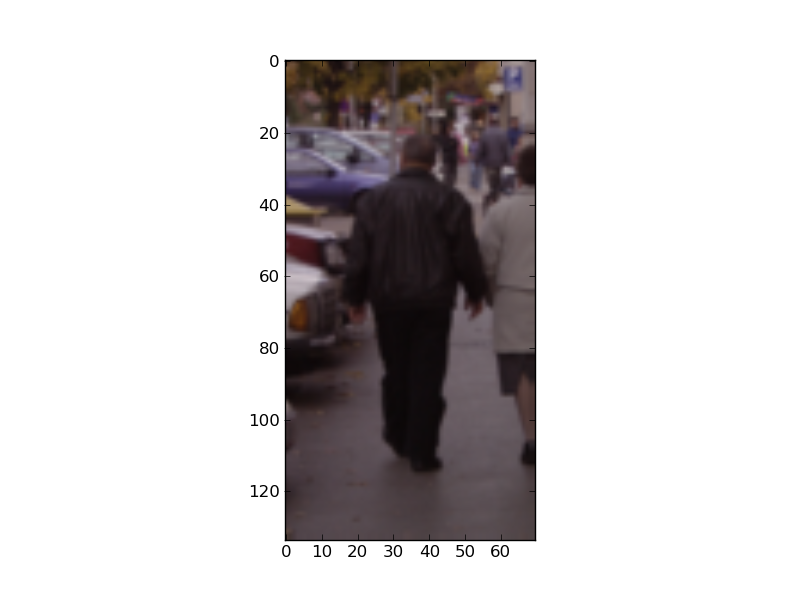
\includegraphics[width=4cm]{dbshow-0-0.png} 
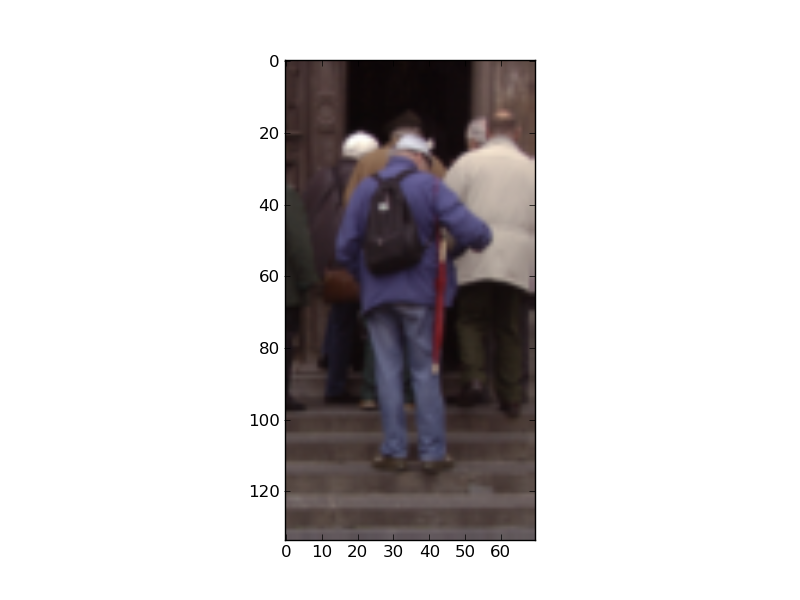
\includegraphics[width=4cm]{dbshow-0-1.png} 
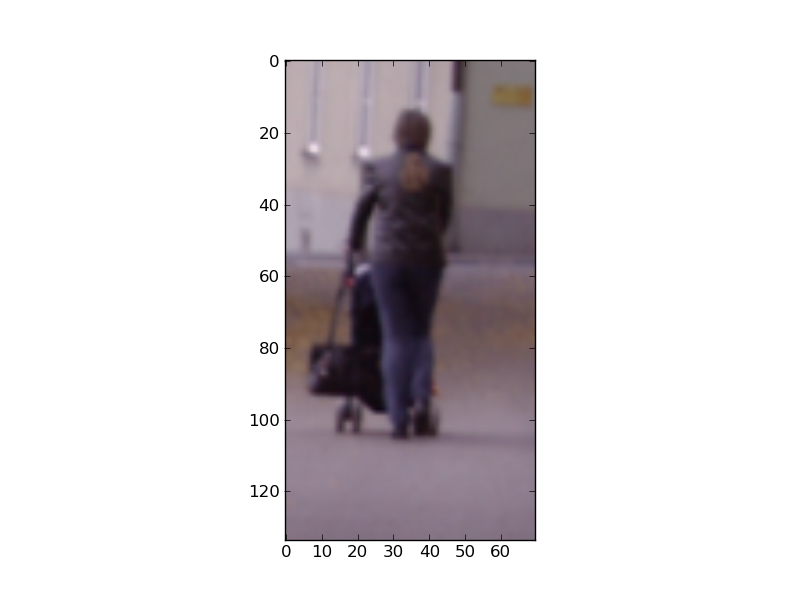
\includegraphics[width=4cm]{dbshow-0-2.png} 
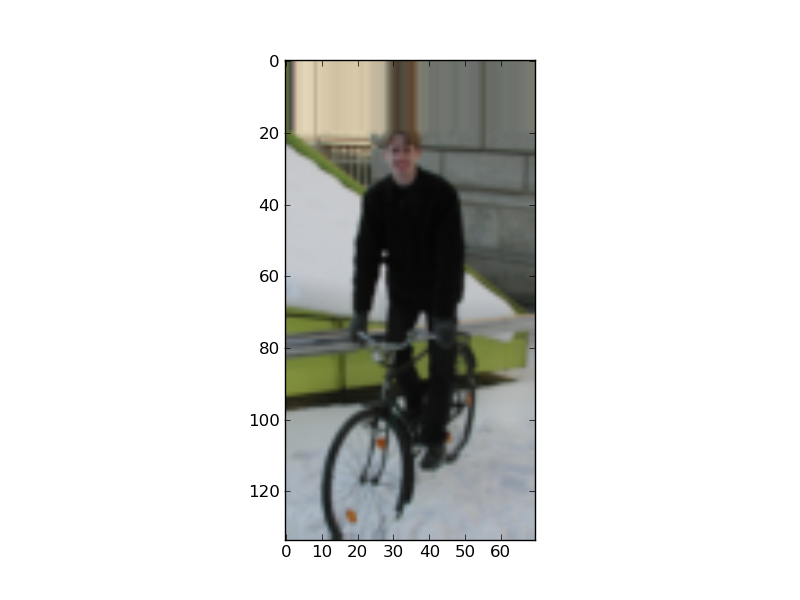
\includegraphics[width=4cm]{dbshow-0-3.png} 
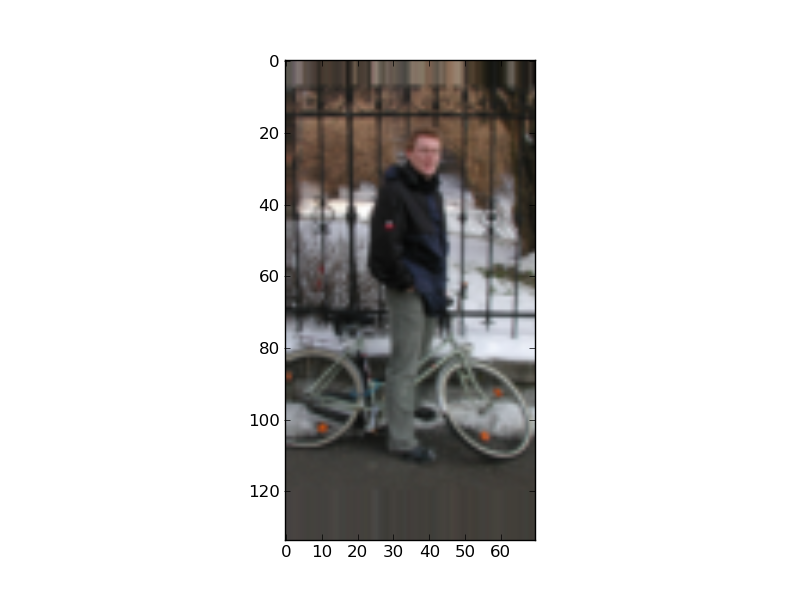
\includegraphics[width=4cm]{dbshow-0-4.png} 
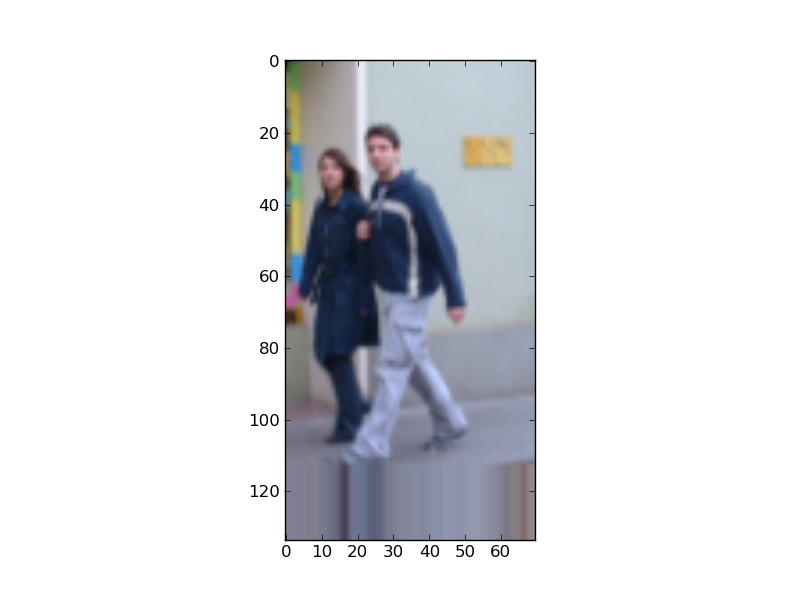
\includegraphics[width=4cm]{dbshow-0-5.png} 
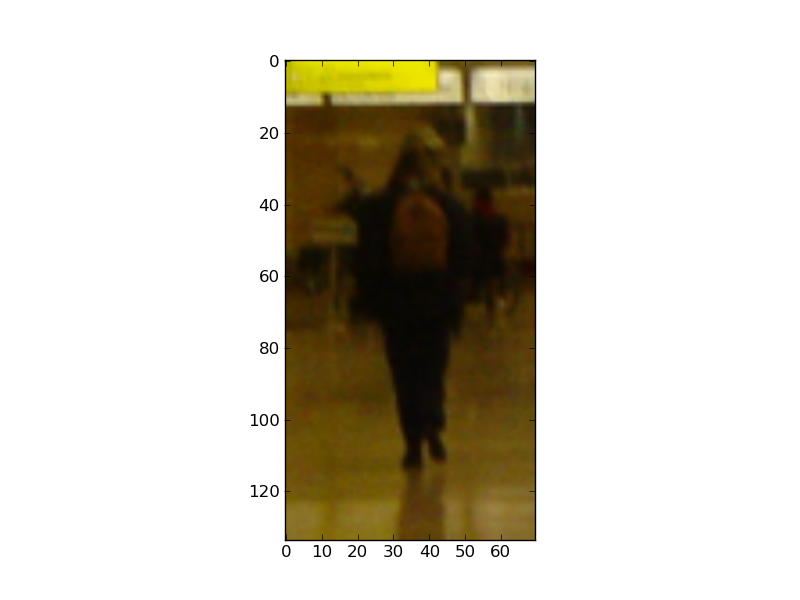
\includegraphics[width=4cm]{dbshow-0-6.png} 
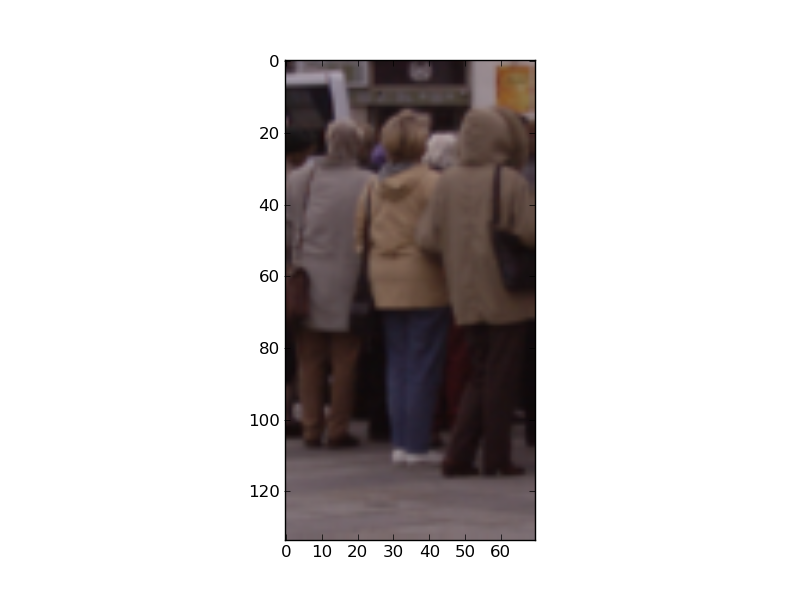
\includegraphics[width=4cm]{dbshow-0-7.png} 
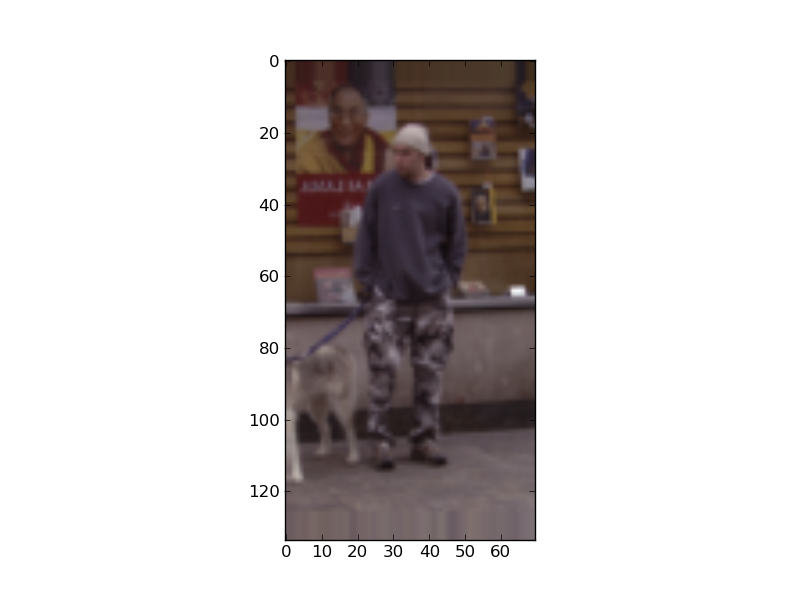
\includegraphics[width=4cm]{dbshow-0-8.png} 
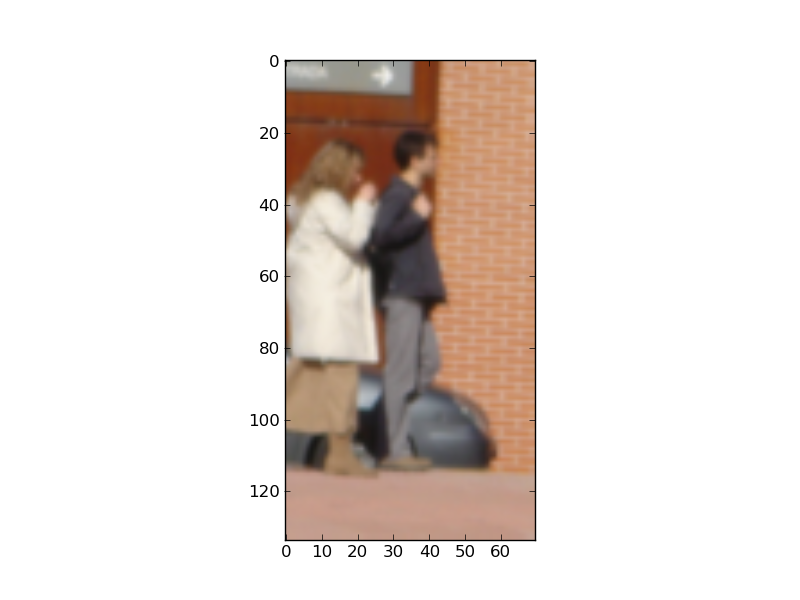
\includegraphics[width=4cm]{dbshow-0-9.png} 















\lstset{
language=bash,                % choose the language of the code
basicstyle=\footnotesize,       % the size of the fonts that are used for the code
numbers=left,                   % where to put the line-numbers
numberstyle=\footnotesize,      % the size of the fonts that are used for the line-numbers
stepnumber=5,                   % the step between two line-numbers. If it's 1 each line will be numbered
numbersep=5pt,                  % how far the line-numbers are from the code
backgroundcolor=\color{white},  % choose the background color. You must add \usepackage{color}
showspaces=false,               % show spaces adding particular underscores
showstringspaces=false,         % underline spaces within strings
showtabs=false,                 % show tabs within strings adding particular underscores
frame=single,	                % adds a frame around the code
tabsize=2,	                % sets default tabsize to 2 spaces
captionpos=b,                   % sets the caption-position to bottom
breaklines=true,                % sets automatic line breaking
breakatwhitespace=false         % sets if automatic breaks should only happen at whitespace
}
\begin{lstlisting}
python dbshow.py --help

\end{lstlisting}






{\small  \tt
\begin{verbatim}
#######################################################################################
Database Viewer
version :0.1
author :Bertrand Nouvel bertrand.nouvel@gmail.com
        COPYRIGHT Bertrand Nouvel - JFLI - CNRS 2009
#######################################################################################
	-h/--help 		:Displays this help message and exit
	--db database		:set the database to be read
	--dbargs database_arguments		:set database options
	--dbhelp 		:show info on parameters required by the database
	-i/--interval interval		:wait for specified interval in-between entries
#######################################################################################


\end{verbatim}
}















\lstset{
language=bash,                % choose the language of the code
basicstyle=\footnotesize,       % the size of the fonts that are used for the code
numbers=left,                   % where to put the line-numbers
numberstyle=\footnotesize,      % the size of the fonts that are used for the line-numbers
stepnumber=5,                   % the step between two line-numbers. If it's 1 each line will be numbered
numbersep=5pt,                  % how far the line-numbers are from the code
backgroundcolor=\color{white},  % choose the background color. You must add \usepackage{color}
showspaces=false,               % show spaces adding particular underscores
showstringspaces=false,         % underline spaces within strings
showtabs=false,                 % show tabs within strings adding particular underscores
frame=single,	                % adds a frame around the code
tabsize=2,	                % sets default tabsize to 2 spaces
captionpos=b,                   % sets the caption-position to bottom
breaklines=true,                % sets automatic line breaking
breakatwhitespace=false         % sets if automatic breaks should only happen at whitespace
}
\begin{lstlisting}
python dbshow.py --db tv2007concept --dbhelp

\end{lstlisting}






{\small  \tt
\begin{verbatim}
Please Install PyEm2
ArgSpec(args=['self', 'conceptname', 'positive', 'randomized', 'videoset'], varargs=None, keywords=None, defaults=('Dog', True, True, 'devel'))


\end{verbatim}
}




It may also be the good moment also to have a look at the code of the application.






\lstset{
language=Python,                % choose the language of the code
basicstyle=\footnotesize,       % the size of the fonts that are used for the code
numbers=left,                   % where to put the line-numbers
numberstyle=\footnotesize,      % the size of the fonts that are used for the line-numbers
stepnumber=5,                   % the step between two line-numbers. If it's 1 each line will be numbered
numbersep=5pt,                  % how far the line-numbers are from the code
backgroundcolor=\color{white},  % choose the background color. You must add \usepackage{color}
showspaces=false,               % show spaces adding particular underscores
showstringspaces=false,         % underline spaces within strings
showtabs=false,                 % show tabs within strings adding particular underscores
frame=single,	                % adds a frame around the code
tabsize=2,	                % sets default tabsize to 2 spaces
captionpos=b,                   % sets the caption-position to bottom
breaklines=true,                % sets automatic line breaking
breakatwhitespace=false         % sets if automatic breaks should only happen at whitespace
}
\begin{lstlisting}
# -*- coding: utf-8 -*-
from pycvf.lib.info.graph import *
from pycvf.core.generic_application import *

class DbShowApp(DatabaseUsingApplication):
  class ProgramMetadata(object):
      name="Database Show Application"
      version="1.0"
      author="Bertrand Nouvel bertrand.nouvel@gmail.com"
      copyright="        COPYRIGHT Bertrand Nouvel - JFLI - CNRS 2009"

  delay=CmdLineString("i","interval","interval","wait for specified interval in-between entries","0")                             

  @classmethod
  def process(cls,nrels=1,*args,**kwargs):
                                                                                       
     delay=float(cls.delay.value)

     for i in cls.vdb:
       cls.vdb.display(i[0])
       if (delay):
          time.sleep(delay)
       
DbShowApp.run(sys.argv[1:])

\end{lstlisting}












This quite informative.

First of all the code contains only the essential informations for the application,


 We are creating an application that will iterate over one database 
 An optional delay is can be passed  
 When iterating over one database received elements are couple made of the form "element", "address"  
 The function is called display, but it is actually a mor generic function that will render a sound if it is a sound and so on 






\section{Evaluation Databases}
\lstset{
language=bash,                % choose the language of the code
basicstyle=\footnotesize,       % the size of the fonts that are used for the code
numbers=left,                   % where to put the line-numbers
numberstyle=\footnotesize,      % the size of the fonts that are used for the line-numbers
stepnumber=5,                   % the step between two line-numbers. If it's 1 each line will be numbered
numbersep=5pt,                  % how far the line-numbers are from the code
backgroundcolor=\color{white},  % choose the background color. You must add \usepackage{color}
showspaces=false,               % show spaces adding particular underscores
showstringspaces=false,         % underline spaces within strings
showtabs=false,                 % show tabs within strings adding particular underscores
frame=single,	                % adds a frame around the code
tabsize=2,	                % sets default tabsize to 2 spaces
captionpos=b,                   % sets the caption-position to bottom
breaklines=true,                % sets automatic line breaking
breakatwhitespace=false         % sets if automatic breaks should only happen at whitespace
}
\begin{lstlisting}
python dbeval.py --db yahoo --dbargs "'query':'tomato'"

\end{lstlisting}









To use an evaluated database you should do :












\lstset{
language=bash,                % choose the language of the code
basicstyle=\footnotesize,       % the size of the fonts that are used for the code
numbers=left,                   % where to put the line-numbers
numberstyle=\footnotesize,      % the size of the fonts that are used for the line-numbers
stepnumber=5,                   % the step between two line-numbers. If it's 1 each line will be numbered
numbersep=5pt,                  % how far the line-numbers are from the code
backgroundcolor=\color{white},  % choose the background color. You must add \usepackage{color}
showspaces=false,               % show spaces adding particular underscores
showstringspaces=false,         % underline spaces within strings
showtabs=false,                 % show tabs within strings adding particular underscores
frame=single,	                % adds a frame around the code
tabsize=2,	                % sets default tabsize to 2 spaces
captionpos=b,                   % sets the caption-position to bottom
breaklines=true,                % sets automatic line breaking
breakatwhitespace=false         % sets if automatic breaks should only happen at whitespace
}
\begin{lstlisting}
python dbshow.py --db user_filtered --dbargs "'db':'yahoo','dbargs':\"'query':'tomato'\""

\end{lstlisting}







It is also possible to query to be evaluated database directly, by using the previous command. 
On the first run, the computer will ask the user to evaluate the database.







\section{Building Simple Indexes}
Simple indexes just associates a content with an address.










\lstset{
language=bash,                % choose the language of the code
basicstyle=\footnotesize,       % the size of the fonts that are used for the code
numbers=left,                   % where to put the line-numbers
numberstyle=\footnotesize,      % the size of the fonts that are used for the line-numbers
stepnumber=5,                   % the step between two line-numbers. If it's 1 each line will be numbered
numbersep=5pt,                  % how far the line-numbers are from the code
backgroundcolor=\color{white},  % choose the background color. You must add \usepackage{color}
showspaces=false,               % show spaces adding particular underscores
showstringspaces=false,         % underline spaces within strings
showtabs=false,                 % show tabs within strings adding particular underscores
frame=single,	                % adds a frame around the code
tabsize=2,	                % sets default tabsize to 2 spaces
captionpos=b,                   % sets the caption-position to bottom
breaklines=true,                % sets automatic line breaking
breakatwhitespace=false         % sets if automatic breaks should only happen at whitespace
}
\begin{lstlisting}
python build_simple_index.pyc -m naive \
 --db image_directory \
 --dbargs "'path' : '/home/tranx/databases/INRIAPerson/70X134H96/Test/pos/', 'rescale':(8,6,'T')" \
 -s "inria"

\end{lstlisting}
















\lstset{
language=bash,                % choose the language of the code
basicstyle=\footnotesize,       % the size of the fonts that are used for the code
numbers=left,                   % where to put the line-numbers
numberstyle=\footnotesize,      % the size of the fonts that are used for the line-numbers
stepnumber=5,                   % the step between two line-numbers. If it's 1 each line will be numbered
numbersep=5pt,                  % how far the line-numbers are from the code
backgroundcolor=\color{white},  % choose the background color. You must add \usepackage{color}
showspaces=false,               % show spaces adding particular underscores
showstringspaces=false,         % underline spaces within strings
showtabs=false,                 % show tabs within strings adding particular underscores
frame=single,	                % adds a frame around the code
tabsize=2,	                % sets default tabsize to 2 spaces
captionpos=b,                   % sets the caption-position to bottom
breaklines=true,                % sets automatic line breaking
breakatwhitespace=false         % sets if automatic breaks should only happen at whitespace
}
\begin{lstlisting}
python build_simple_index.pyc -m naive \
 --db imgkanji --dbargs "'scl':(16,16)" 

\end{lstlisting}
















\lstset{
language=bash,                % choose the language of the code
basicstyle=\footnotesize,       % the size of the fonts that are used for the code
numbers=left,                   % where to put the line-numbers
numberstyle=\footnotesize,      % the size of the fonts that are used for the line-numbers
stepnumber=5,                   % the step between two line-numbers. If it's 1 each line will be numbered
numbersep=5pt,                  % how far the line-numbers are from the code
backgroundcolor=\color{white},  % choose the background color. You must add \usepackage{color}
showspaces=false,               % show spaces adding particular underscores
showstringspaces=false,         % underline spaces within strings
showtabs=false,                 % show tabs within strings adding particular underscores
frame=single,	                % adds a frame around the code
tabsize=2,	                % sets default tabsize to 2 spaces
captionpos=b,                   % sets the caption-position to bottom
breaklines=true,                % sets automatic line breaking
breakatwhitespace=false         % sets if automatic breaks should only happen at whitespace
}
\begin{lstlisting}
python gcbquery.pyc \
   -m naive \
   --db image_directory \
    --dbargs "'path' : '/home/tranx/databases/INRIAPerson/70X134H96/Test/pos', 'rescale':(8,6,'T')"\
    -s "inria" \
    -i 1 -b 30 -n 5

\end{lstlisting}




















\lstset{
language=bash,                % choose the language of the code
basicstyle=\footnotesize,       % the size of the fonts that are used for the code
numbers=left,                   % where to put the line-numbers
numberstyle=\footnotesize,      % the size of the fonts that are used for the line-numbers
stepnumber=5,                   % the step between two line-numbers. If it's 1 each line will be numbered
numbersep=5pt,                  % how far the line-numbers are from the code
backgroundcolor=\color{white},  % choose the background color. You must add \usepackage{color}
showspaces=false,               % show spaces adding particular underscores
showstringspaces=false,         % underline spaces within strings
showtabs=false,                 % show tabs within strings adding particular underscores
frame=single,	                % adds a frame around the code
tabsize=2,	                % sets default tabsize to 2 spaces
captionpos=b,                   % sets the caption-position to bottom
breaklines=true,                % sets automatic line breaking
breakatwhitespace=false         % sets if automatic breaks should only happen at whitespace
}
\begin{lstlisting}
python build_simple_index.py -m naive  --db imgkanji --dbargs "'scl':(16,16),'fontsz('12')'" -s kanji12
python nearestneighborapp.py -m naive  --db imgkanji --dbargs "'scl':(16,16),'fontsz('12')'" -s kanji12

\end{lstlisting}





\section{Using Models}
\subsection{Checking the Outputs of Models}
Once you have defined a model, it is first important to check  what models

To automatically view all the important features of a model you may use model\_features\_view.py:









\lstset{
language=bash,                % choose the language of the code
basicstyle=\footnotesize,       % the size of the fonts that are used for the code
numbers=left,                   % where to put the line-numbers
numberstyle=\footnotesize,      % the size of the fonts that are used for the line-numbers
stepnumber=5,                   % the step between two line-numbers. If it's 1 each line will be numbered
numbersep=5pt,                  % how far the line-numbers are from the code
backgroundcolor=\color{white},  % choose the background color. You must add \usepackage{color}
showspaces=false,               % show spaces adding particular underscores
showstringspaces=false,         % underline spaces within strings
showtabs=false,                 % show tabs within strings adding particular underscores
frame=single,	                % adds a frame around the code
tabsize=2,	                % sets default tabsize to 2 spaces
captionpos=b,                   % sets the caption-position to bottom
breaklines=true,                % sets automatic line breaking
breakatwhitespace=false         % sets if automatic breaks should only happen at whitespace
}
\begin{lstlisting}
python model_features_view.py \
 -db imgkanji \
  -m "#M('naive')|{'a':M('image.sift')|{'b':M('basics.mean')}}"

\end{lstlisting}










Although this allow to graphically check, your features this does not allow
you yet to display informations as they will be passed to your machine learning algorithms.
For this you have to select a path and a structure












\lstset{
language=bash,                % choose the language of the code
basicstyle=\footnotesize,       % the size of the fonts that are used for the code
numbers=left,                   % where to put the line-numbers
numberstyle=\footnotesize,      % the size of the fonts that are used for the line-numbers
stepnumber=5,                   % the step between two line-numbers. If it's 1 each line will be numbered
numbersep=5pt,                  % how far the line-numbers are from the code
backgroundcolor=\color{white},  % choose the background color. You must add \usepackage{color}
showspaces=false,               % show spaces adding particular underscores
showstringspaces=false,         % underline spaces within strings
showtabs=false,                 % show tabs within strings adding particular underscores
frame=single,	                % adds a frame around the code
tabsize=2,	                % sets default tabsize to 2 spaces
captionpos=b,                   % sets the caption-position to bottom
breaklines=true,                % sets automatic line breaking
breakatwhitespace=false         % sets if automatic breaks should only happen at whitespace
}
\begin{lstlisting}
python model_feature_print_path.\
 -db imgkanji \
  -m "#M('naive')|{'a':M('image.sift')|{'b':M('basics.mean')}}" \
  --modelpart "//a/b"

\end{lstlisting}
















\lstset{
language=bash,                % choose the language of the code
basicstyle=\footnotesize,       % the size of the fonts that are used for the code
numbers=left,                   % where to put the line-numbers
numberstyle=\footnotesize,      % the size of the fonts that are used for the line-numbers
stepnumber=5,                   % the step between two line-numbers. If it's 1 each line will be numbered
numbersep=5pt,                  % how far the line-numbers are from the code
backgroundcolor=\color{white},  % choose the background color. You must add \usepackage{color}
showspaces=false,               % show spaces adding particular underscores
showstringspaces=false,         % underline spaces within strings
showtabs=false,                 % show tabs within strings adding particular underscores
frame=single,	                % adds a frame around the code
tabsize=2,	                % sets default tabsize to 2 spaces
captionpos=b,                   % sets the caption-position to bottom
breaklines=true,                % sets automatic line breaking
breakatwhitespace=false         % sets if automatic breaks should only happen at whitespace
}
\begin{lstlisting}
python model_feature_print_path.py\
 -db imgkanji \
  -m "#M('naive')|{'a':M('image.sift')|{'b':M('basics.mean')}}" \
   --modelpart "//#pixels"

\end{lstlisting}















\lstset{
language=bash,                % choose the language of the code
basicstyle=\footnotesize,       % the size of the fonts that are used for the code
numbers=left,                   % where to put the line-numbers
numberstyle=\footnotesize,      % the size of the fonts that are used for the line-numbers
stepnumber=5,                   % the step between two line-numbers. If it's 1 each line will be numbered
numbersep=5pt,                  % how far the line-numbers are from the code
backgroundcolor=\color{white},  % choose the background color. You must add \usepackage{color}
showspaces=false,               % show spaces adding particular underscores
showstringspaces=false,         % underline spaces within strings
showtabs=false,                 % show tabs within strings adding particular underscores
frame=single,	                % adds a frame around the code
tabsize=2,	                % sets default tabsize to 2 spaces
captionpos=b,                   % sets the caption-position to bottom
breaklines=true,                % sets automatic line breaking
breakatwhitespace=false         % sets if automatic breaks should only happen at whitespace
}
\begin{lstlisting}
python model_feature_print_path.py\
 -db imgkanji \
  --dbargs '"scl":(16,16)' \
  -m "#M('naive')|{'a':M('image.sift')|{'b':M('basics.mean')}}" \
  --modelpart "/#monochrome-V4*" \\

\end{lstlisting}















\lstset{
language=bash,                % choose the language of the code
basicstyle=\footnotesize,       % the size of the fonts that are used for the code
numbers=left,                   % where to put the line-numbers
numberstyle=\footnotesize,      % the size of the fonts that are used for the line-numbers
stepnumber=5,                   % the step between two line-numbers. If it's 1 each line will be numbered
numbersep=5pt,                  % how far the line-numbers are from the code
backgroundcolor=\color{white},  % choose the background color. You must add \usepackage{color}
showspaces=false,               % show spaces adding particular underscores
showstringspaces=false,         % underline spaces within strings
showtabs=false,                 % show tabs within strings adding particular underscores
frame=single,	                % adds a frame around the code
tabsize=2,	                % sets default tabsize to 2 spaces
captionpos=b,                   % sets the caption-position to bottom
breaklines=true,                % sets automatic line breaking
breakatwhitespace=false         % sets if automatic breaks should only happen at whitespace
}
\begin{lstlisting}
python model_feature_print_path.py \\
   --db imgkanji --modelpart "//a#pointlist" --dbargs '"scl":(48,48)' \\
    -m "#M('naive')|{'a':(M('image.sift')|{'b':M('basics.mean')})*{'pointlist':S(('list.PointListStructure',('NNP',[2])))} }"

\end{lstlisting}















\lstset{
language=bash,                % choose the language of the code
basicstyle=\footnotesize,       % the size of the fonts that are used for the code
numbers=left,                   % where to put the line-numbers
numberstyle=\footnotesize,      % the size of the fonts that are used for the line-numbers
stepnumber=5,                   % the step between two line-numbers. If it's 1 each line will be numbered
numbersep=5pt,                  % how far the line-numbers are from the code
backgroundcolor=\color{white},  % choose the background color. You must add \usepackage{color}
showspaces=false,               % show spaces adding particular underscores
showstringspaces=false,         % underline spaces within strings
showtabs=false,                 % show tabs within strings adding particular underscores
frame=single,	                % adds a frame around the code
tabsize=2,	                % sets default tabsize to 2 spaces
captionpos=b,                   % sets the caption-position to bottom
breaklines=true,                % sets automatic line breaking
breakatwhitespace=false         % sets if automatic breaks should only happen at whitespace
}
\begin{lstlisting}
python model_feature_print_path.py \\
   --db imgkanji --modelpart "//a#pointlist/mean" --dbargs '"scl":(48,48)' \\
    -m "#M('naive')|{'a':(M('image.sift')|{'b':M('basics.mean')})*{'pointlist':S(('list.PointListStructure',('NNP',[2])))} }"

\end{lstlisting}




By using the "@" operator it is possible to retrieve address associated with a structure :









\lstset{
language=bash,                % choose the language of the code
basicstyle=\footnotesize,       % the size of the fonts that are used for the code
numbers=left,                   % where to put the line-numbers
numberstyle=\footnotesize,      % the size of the fonts that are used for the line-numbers
stepnumber=5,                   % the step between two line-numbers. If it's 1 each line will be numbered
numbersep=5pt,                  % how far the line-numbers are from the code
backgroundcolor=\color{white},  % choose the background color. You must add \usepackage{color}
showspaces=false,               % show spaces adding particular underscores
showstringspaces=false,         % underline spaces within strings
showtabs=false,                 % show tabs within strings adding particular underscores
frame=single,	                % adds a frame around the code
tabsize=2,	                % sets default tabsize to 2 spaces
captionpos=b,                   % sets the caption-position to bottom
breaklines=true,                % sets automatic line breaking
breakatwhitespace=false         % sets if automatic breaks should only happen at whitespace
}
\begin{lstlisting}
python model_feature_print_path.py \\
   --db imgkanji --dbargs '"scl":(16,16)' \\
   -m "#M('naive')" \\
   --modelpart "/#color-V4@" 

\end{lstlisting}
















\lstset{
language=bash,                % choose the language of the code
basicstyle=\footnotesize,       % the size of the fonts that are used for the code
numbers=left,                   % where to put the line-numbers
numberstyle=\footnotesize,      % the size of the fonts that are used for the line-numbers
stepnumber=5,                   % the step between two line-numbers. If it's 1 each line will be numbered
numbersep=5pt,                  % how far the line-numbers are from the code
backgroundcolor=\color{white},  % choose the background color. You must add \usepackage{color}
showspaces=false,               % show spaces adding particular underscores
showstringspaces=false,         % underline spaces within strings
showtabs=false,                 % show tabs within strings adding particular underscores
frame=single,	                % adds a frame around the code
tabsize=2,	                % sets default tabsize to 2 spaces
captionpos=b,                   % sets the caption-position to bottom
breaklines=true,                % sets automatic line breaking
breakatwhitespace=false         % sets if automatic breaks should only happen at whitespace
}
\begin{lstlisting}
python model_feature_print_path.py \\
   --db tv2007concept --dbargs "'conceptname':'Singing'" \\
   -m "#M('naive')" \\
   --modelpart "/#images/#color-V4@" 

\end{lstlisting}















\lstset{
language=bash,                % choose the language of the code
basicstyle=\footnotesize,       % the size of the fonts that are used for the code
numbers=left,                   % where to put the line-numbers
numberstyle=\footnotesize,      % the size of the fonts that are used for the line-numbers
stepnumber=5,                   % the step between two line-numbers. If it's 1 each line will be numbered
numbersep=5pt,                  % how far the line-numbers are from the code
backgroundcolor=\color{white},  % choose the background color. You must add \usepackage{color}
showspaces=false,               % show spaces adding particular underscores
showstringspaces=false,         % underline spaces within strings
showtabs=false,                 % show tabs within strings adding particular underscores
frame=single,	                % adds a frame around the code
tabsize=2,	                % sets default tabsize to 2 spaces
captionpos=b,                   % sets the caption-position to bottom
breaklines=true,                % sets automatic line breaking
breakatwhitespace=false         % sets if automatic breaks should only happen at whitespace
}
\begin{lstlisting}
python model_feature_print_path.py \\
   --db tv2007concept --dbargs "'conceptname':'Singing'" \\
   -m "#M('naive')|{'#images':MS('images','naive')|{'rescale':M('image.rescaled',(2,2,'T'))}}" \\
   --modelpart "/#images/rescale"

\end{lstlisting}
















\lstset{
language=bash,                % choose the language of the code
basicstyle=\footnotesize,       % the size of the fonts that are used for the code
numbers=left,                   % where to put the line-numbers
numberstyle=\footnotesize,      % the size of the fonts that are used for the line-numbers
stepnumber=5,                   % the step between two line-numbers. If it's 1 each line will be numbered
numbersep=5pt,                  % how far the line-numbers are from the code
backgroundcolor=\color{white},  % choose the background color. You must add \usepackage{color}
showspaces=false,               % show spaces adding particular underscores
showstringspaces=false,         % underline spaces within strings
showtabs=false,                 % show tabs within strings adding particular underscores
frame=single,	                % adds a frame around the code
tabsize=2,	                % sets default tabsize to 2 spaces
captionpos=b,                   % sets the caption-position to bottom
breaklines=true,                % sets automatic line breaking
breakatwhitespace=false         % sets if automatic breaks should only happen at whitespace
}
\begin{lstlisting}
#
# Let's index images inside of the video 
#
TV2007DIR=~/databases/tv2007.meta.sav/ python build_index.py \\
 --db tv2007concept --dbargs "'conceptname':'Singing'" \\
 -m "#M('naive')
      |{'#images':MS('images','naive')
                  |{'rescale':M('image.rescaled',(2,2,'T'))}
       } " \\
 --key "/#images/rescale"  --value "/#images@" --idx index_vectors

\end{lstlisting}
















\lstset{
language=bash,                % choose the language of the code
basicstyle=\footnotesize,       % the size of the fonts that are used for the code
numbers=left,                   % where to put the line-numbers
numberstyle=\footnotesize,      % the size of the fonts that are used for the line-numbers
stepnumber=5,                   % the step between two line-numbers. If it's 1 each line will be numbered
numbersep=5pt,                  % how far the line-numbers are from the code
backgroundcolor=\color{white},  % choose the background color. You must add \usepackage{color}
showspaces=false,               % show spaces adding particular underscores
showstringspaces=false,         % underline spaces within strings
showtabs=false,                 % show tabs within strings adding particular underscores
frame=single,	                % adds a frame around the code
tabsize=2,	                % sets default tabsize to 2 spaces
captionpos=b,                   % sets the caption-position to bottom
breaklines=true,                % sets automatic line breaking
breakatwhitespace=false         % sets if automatic breaks should only happen at whitespace
}
\begin{lstlisting}
#
# May we want something different
#
TV2007DIR=~/databases/tv2007.meta.sav/ python build_index.py \\
 --db tv2007concept --dbargs "'conceptname':'Singing'" \\
 -m "#M('naive')
      |{'#images':MS('images','naive')
                  |{'rescale':M('image.rescaled',(2,2,'T'))}
       } " \\
 --value "/#images/rescale"  --key "/#images@[-1]" --idx index_generic

\end{lstlisting}
















\lstset{
language=bash,                % choose the language of the code
basicstyle=\footnotesize,       % the size of the fonts that are used for the code
numbers=left,                   % where to put the line-numbers
numberstyle=\footnotesize,      % the size of the fonts that are used for the line-numbers
stepnumber=5,                   % the step between two line-numbers. If it's 1 each line will be numbered
numbersep=5pt,                  % how far the line-numbers are from the code
backgroundcolor=\color{white},  % choose the background color. You must add \usepackage{color}
showspaces=false,               % show spaces adding particular underscores
showstringspaces=false,         % underline spaces within strings
showtabs=false,                 % show tabs within strings adding particular underscores
frame=single,	                % adds a frame around the code
tabsize=2,	                % sets default tabsize to 2 spaces
captionpos=b,                   % sets the caption-position to bottom
breaklines=true,                % sets automatic line breaking
breakatwhitespace=false         % sets if automatic breaks should only happen at whitespace
}
\begin{lstlisting}
#
# May we want something different
#
python build_index.py \\
 --db imgkanji --dbargs '"scl":(48,48)'  \\
 -m "#M('naive')
      |{'a':M('image.sift')
             *{'pointlist':S(('list.PointListStructure',('NNP',[2])))}
             |{'#pointlist':MS('pointlist','basics.pcared',16)}
             |{'pointliststat':M('basics.transformedpath',) )

       }" \\
 --value "/a"  --key "/a/" \\
 --idx index_generic

\end{lstlisting}


















\lstset{
language=bash,                % choose the language of the code
basicstyle=\footnotesize,       % the size of the fonts that are used for the code
numbers=left,                   % where to put the line-numbers
numberstyle=\footnotesize,      % the size of the fonts that are used for the line-numbers
stepnumber=5,                   % the step between two line-numbers. If it's 1 each line will be numbered
numbersep=5pt,                  % how far the line-numbers are from the code
backgroundcolor=\color{white},  % choose the background color. You must add \usepackage{color}
showspaces=false,               % show spaces adding particular underscores
showstringspaces=false,         % underline spaces within strings
showtabs=false,                 % show tabs within strings adding particular underscores
frame=single,	                % adds a frame around the code
tabsize=2,	                % sets default tabsize to 2 spaces
captionpos=b,                   % sets the caption-position to bottom
breaklines=true,                % sets automatic line breaking
breakatwhitespace=false         % sets if automatic breaks should only happen at whitespace
}
\begin{lstlisting}
python build_index.py \\
   --db imgkanji  --dbargs '"scl":(48,48)' \\
   -m "#M('naive')|{'a':(M('image.sift')|{'b':M('basics.mean')})*{'pointlist':S(('list.PointListStructure',('NNP',[2])))} }" \\
   --key "//a#pointlist/mean" \\ 
   --value "//a#pointlist@" \\
   -s "position according to mean sift"

\end{lstlisting}
















\lstset{
language=bash,                % choose the language of the code
basicstyle=\footnotesize,       % the size of the fonts that are used for the code
numbers=left,                   % where to put the line-numbers
numberstyle=\footnotesize,      % the size of the fonts that are used for the line-numbers
stepnumber=5,                   % the step between two line-numbers. If it's 1 each line will be numbered
numbersep=5pt,                  % how far the line-numbers are from the code
backgroundcolor=\color{white},  % choose the background color. You must add \usepackage{color}
showspaces=false,               % show spaces adding particular underscores
showstringspaces=false,         % underline spaces within strings
showtabs=false,                 % show tabs within strings adding particular underscores
frame=single,	                % adds a frame around the code
tabsize=2,	                % sets default tabsize to 2 spaces
captionpos=b,                   % sets the caption-position to bottom
breaklines=true,                % sets automatic line breaking
breakatwhitespace=false         % sets if automatic breaks should only happen at whitespace
}
\begin{lstlisting}
python gsquery.py \\
   --db imgkanji  --dbargs '"scl":(48,48)' \\
   -m "#M('naive')|{'a':(M('image.sift')|{'b':M('basics.mean')})*{'pointlist':S(('list.PointListStructure',('NNP',[2])))} }" \\
   --key "//a#pointlist/mean" \\
   --value "//a#pointlist@" \\
    -s "position according to mean sift"

\end{lstlisting}

















\section{Training and Testing Models}
Loading a model




\lstset{
language=Python,                % choose the language of the code
basicstyle=\footnotesize,       % the size of the fonts that are used for the code
numbers=left,                   % where to put the line-numbers
numberstyle=\footnotesize,      % the size of the fonts that are used for the line-numbers
stepnumber=5,                   % the step between two line-numbers. If it's 1 each line will be numbered
numbersep=5pt,                  % how far the line-numbers are from the code
backgroundcolor=\color{white},  % choose the background color. You must add \usepackage{color}
showspaces=false,               % show spaces adding particular underscores
showstringspaces=false,         % underline spaces within strings
showtabs=false,                 % show tabs within strings adding particular underscores
frame=single,	                % adds a frame around the code
tabsize=2,	                % sets default tabsize to 2 spaces
captionpos=b,                   % sets the caption-position to bottom
breaklines=true,                % sets automatic line breaking
breakatwhitespace=false         % sets if automatic breaks should only happen at whitespace
}
\begin{lstlisting}
from pycvf.models.modelbuilder import model_build
from pycvf.databases.mvp import ContentsDatabase
db=ContentsDatabase()
m=model_build("#M('naive')",db)
m.get_cnames()
m.get_cnames_models()
m.print_tree()
m.get_by_name("//")
m.get_default_structure()
e=iter(db).next()
len(e[0])
m.get_default_structure()



ds=m.get_default_structure()[0]
m=ds.shape(e[0])
ds.cliques_addresses(e[0],'Elements') # get your keys 


r0=ds.instantiate_map(m,numpy.float)
r1=ds.map(numpy.mean,e[0])



r0=ds.instantiate_map(m,object)
##
## DO INDEX MAPPING
##

ds.cliques_extract_all(e[0],'Elements') # get your valus
ds.cliques_extract_all(e[0],'Elements') #
for_instance(e)

\end{lstlisting}













Simple indexes just associates a content with an address.










\lstset{
language=bash,                % choose the language of the code
basicstyle=\footnotesize,       % the size of the fonts that are used for the code
numbers=left,                   % where to put the line-numbers
numberstyle=\footnotesize,      % the size of the fonts that are used for the line-numbers
stepnumber=5,                   % the step between two line-numbers. If it's 1 each line will be numbered
numbersep=5pt,                  % how far the line-numbers are from the code
backgroundcolor=\color{white},  % choose the background color. You must add \usepackage{color}
showspaces=false,               % show spaces adding particular underscores
showstringspaces=false,         % underline spaces within strings
showtabs=false,                 % show tabs within strings adding particular underscores
frame=single,	                % adds a frame around the code
tabsize=2,	                % sets default tabsize to 2 spaces
captionpos=b,                   % sets the caption-position to bottom
breaklines=true,                % sets automatic line breaking
breakatwhitespace=false         % sets if automatic breaks should only happen at whitespace
}
\begin{lstlisting}
python train_model.pyc -m '#M("naive")-{"mean":L("meanvariancemodel.SimpleMeanVarianceModel")}' \
 --db image_directory \
 --dbargs "'path' : '/home/tranx/databases/INRIAPerson/70X134H96/Test/pos/', 'rescale':(8,6,'T')" \
 -s "inria-naive-mean"

\end{lstlisting}







\begin{verbatim}
saving model <jfli.models.naive.MyModel object at 0x4a7bf10>
saving model structure ('horizontal-edges', (<jfli.models.structures.spatial.SpatialStructure instance at 0x4a50a70>, ('H', '')))FAILED
saving model structure ('color-pixels', <jfli.models.structures.spatial.SpatialStructure instance at 0x4a50710>)FAILED
saving model structure ('datas', <jfli.models.structures.spatial.SpatialStructure instance at 0x4a50680>)FAILED
saving model structure ('vertical-edges', (<jfli.models.structures.spatial.SpatialStructure instance at 0x4a50ab8>, ('V', '')))FAILED
saving model statmodels ('mean', <jfli.stats.cachedmodel.CachedModel instance at 0x4a50b00>)writing /home/tranx/models/MnaivemeanLmeanvariancemodelSimpleMeanVarianceModel-image_directory-inria-naive-mean//mean/lowlevel...

\end{verbatim}












\lstset{
language=bash,                % choose the language of the code
basicstyle=\footnotesize,       % the size of the fonts that are used for the code
numbers=left,                   % where to put the line-numbers
numberstyle=\footnotesize,      % the size of the fonts that are used for the line-numbers
stepnumber=5,                   % the step between two line-numbers. If it's 1 each line will be numbered
numbersep=5pt,                  % how far the line-numbers are from the code
backgroundcolor=\color{white},  % choose the background color. You must add \usepackage{color}
showspaces=false,               % show spaces adding particular underscores
showstringspaces=false,         % underline spaces within strings
showtabs=false,                 % show tabs within strings adding particular underscores
frame=single,	                % adds a frame around the code
tabsize=2,	                % sets default tabsize to 2 spaces
captionpos=b,                   % sets the caption-position to bottom
breaklines=true,                % sets automatic line breaking
breakatwhitespace=false         % sets if automatic breaks should only happen at whitespace
}
\begin{lstlisting}
python test_model.pyc \
   -m naive \
   --db image_directory \
    --dbargs "'path' : '/home/tranx/databases/INRIAPerson/70X134H96/Test/pos', 'rescale':(8,6,'T')" \
    -s "inria" \

\end{lstlisting}





\section{Learning Skin Color And Doing Skin Color Filtering}
\lstset{
language=bash,                % choose the language of the code
basicstyle=\footnotesize,       % the size of the fonts that are used for the code
numbers=left,                   % where to put the line-numbers
numberstyle=\footnotesize,      % the size of the fonts that are used for the line-numbers
stepnumber=5,                   % the step between two line-numbers. If it's 1 each line will be numbered
numbersep=5pt,                  % how far the line-numbers are from the code
backgroundcolor=\color{white},  % choose the background color. You must add \usepackage{color}
showspaces=false,               % show spaces adding particular underscores
showstringspaces=false,         % underline spaces within strings
showtabs=false,                 % show tabs within strings adding particular underscores
frame=single,	                % adds a frame around the code
tabsize=2,	                % sets default tabsize to 2 spaces
captionpos=b,                   % sets the caption-position to bottom
breaklines=true,                % sets automatic line breaking
breakatwhitespace=false         % sets if automatic breaks should only happen at whitespace
}
\begin{lstlisting}
python dbshow.py \
    --db image_directory \
    --dbargs "'path' : '/home/tranx/databases/anzen_zeitaku/skins/','rescale':(32,32,'T')" 

\end{lstlisting}








\noindent
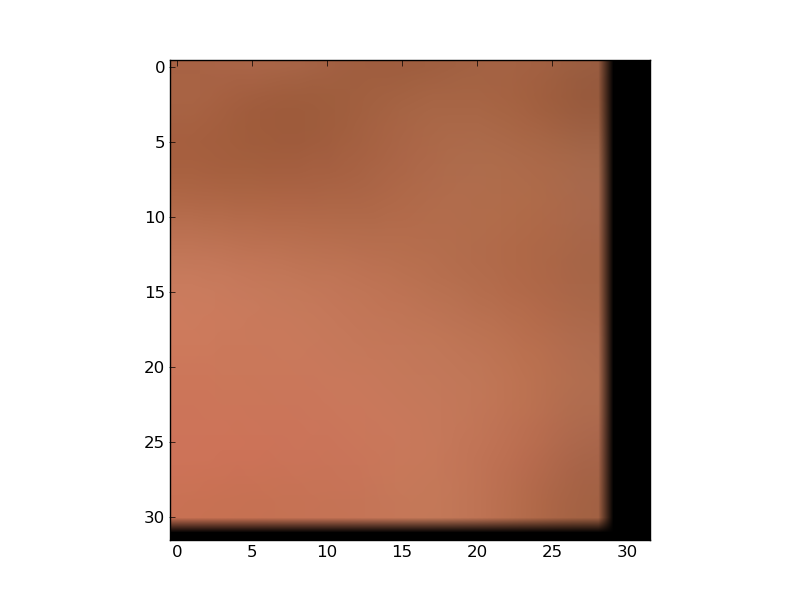
\includegraphics[width=4cm]{dbshow-1-0.png} 
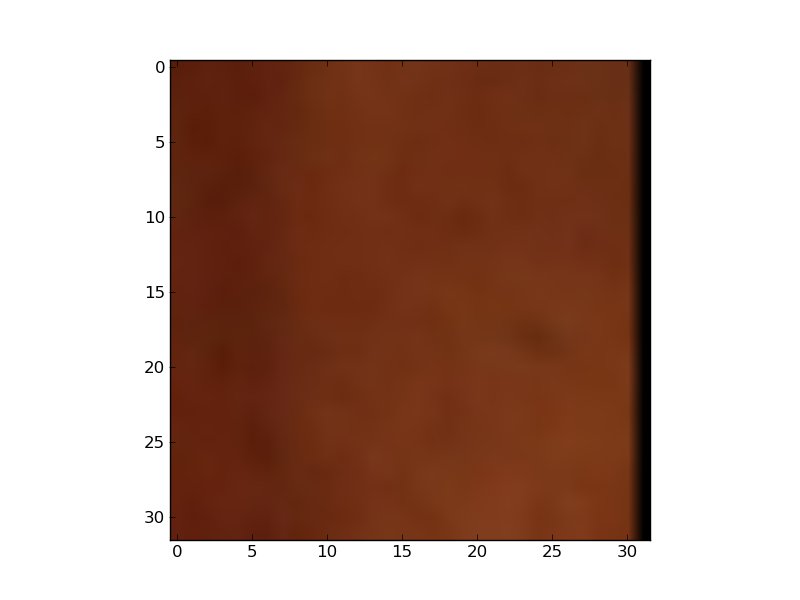
\includegraphics[width=4cm]{dbshow-1-1.png} 
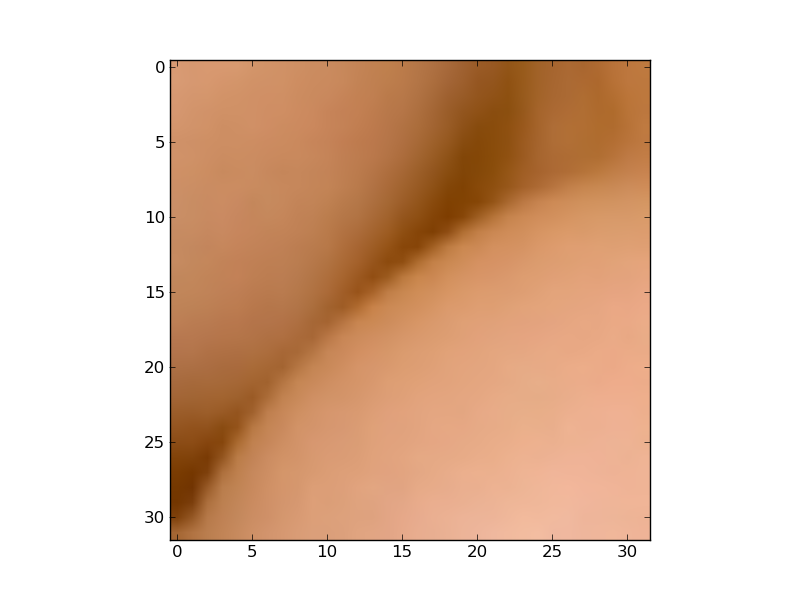
\includegraphics[width=4cm]{dbshow-1-2.png} 
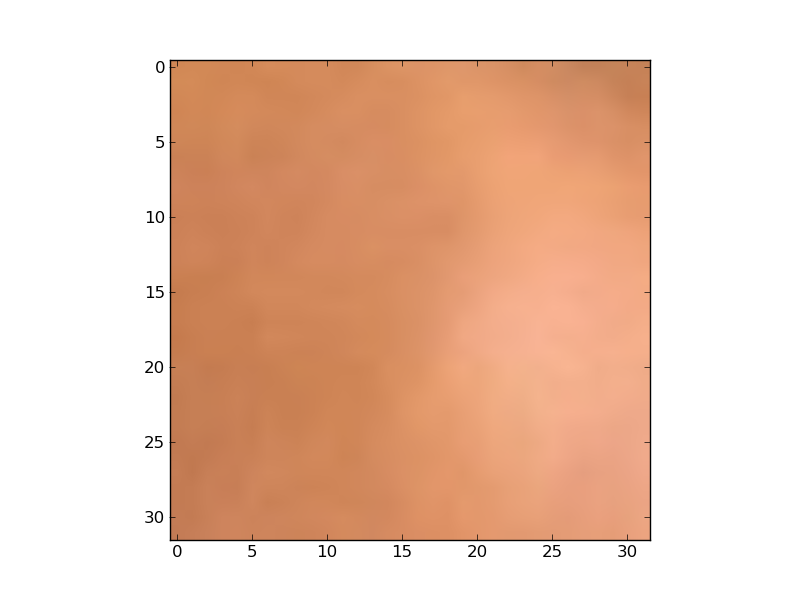
\includegraphics[width=4cm]{dbshow-1-3.png} 
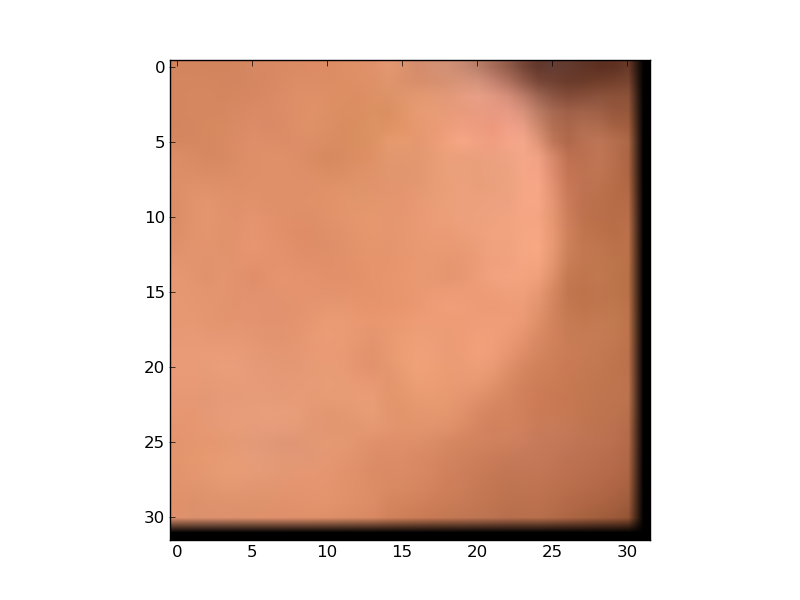
\includegraphics[width=4cm]{dbshow-1-4.png} 













\lstset{
language=bash,                % choose the language of the code
basicstyle=\footnotesize,       % the size of the fonts that are used for the code
numbers=left,                   % where to put the line-numbers
numberstyle=\footnotesize,      % the size of the fonts that are used for the line-numbers
stepnumber=5,                   % the step between two line-numbers. If it's 1 each line will be numbered
numbersep=5pt,                  % how far the line-numbers are from the code
backgroundcolor=\color{white},  % choose the background color. You must add \usepackage{color}
showspaces=false,               % show spaces adding particular underscores
showstringspaces=false,         % underline spaces within strings
showtabs=false,                 % show tabs within strings adding particular underscores
frame=single,	                % adds a frame around the code
tabsize=2,	                % sets default tabsize to 2 spaces
captionpos=b,                   % sets the caption-position to bottom
breaklines=true,                % sets automatic line breaking
breakatwhitespace=false         % sets if automatic breaks should only happen at whitespace
}
\begin{lstlisting}
python train_model.py \
    -m "#M('naive')
        -{'mean':LS('meanvariancemodel.SimpleMeanVarianceModel','pixels')}" \
    --db image_directory \
    --dbargs "'path' : '/home/tranx/databases/anzen_zeitaku/skins/','rescale':(32,32,'T')" \
    -s "skincolor" 

\end{lstlisting}






This code is roughly equivalent to :










\lstset{
language=bash,                % choose the language of the code
basicstyle=\footnotesize,       % the size of the fonts that are used for the code
numbers=left,                   % where to put the line-numbers
numberstyle=\footnotesize,      % the size of the fonts that are used for the line-numbers
stepnumber=5,                   % the step between two line-numbers. If it's 1 each line will be numbered
numbersep=5pt,                  % how far the line-numbers are from the code
backgroundcolor=\color{white},  % choose the background color. You must add \usepackage{color}
showspaces=false,               % show spaces adding particular underscores
showstringspaces=false,         % underline spaces within strings
showtabs=false,                 % show tabs within strings adding particular underscores
frame=single,	                % adds a frame around the code
tabsize=2,	                % sets default tabsize to 2 spaces
captionpos=b,                   % sets the caption-position to bottom
breaklines=true,                % sets automatic line breaking
breakatwhitespace=false         % sets if automatic breaks should only happen at whitespace
}
\begin{lstlisting}
python train_model.py \
    -m "#M('naive')
        |{'#pixels':MS('color-pixels','naive')  
           -{'mean':L('meanvariancemodel.SimpleMeanVarianceModel')}
         }" \
    --db image_directory \
    --dbargs "'path' : '/home/tranx/databases/anzen_zeitaku/skins/','rescale':(32,32,'T')" \
    -s "skincolor" 

\end{lstlisting}






Now we can verify that we learned the correct color:





\begin{minipage}{\textwidth}
{\small
% Generator: GNU source-highlight, by Lorenzo Bettini, http://www.gnu.org/software/src-highlite
\noindent
\mbox{}\textbf{from}\ jfli.stats.meanvariancemodel\ \textbf{import}\ SimpleMeanVarianceModel\ as\ smvm \\
\mbox{}r=smvm.\textbf{load}(\textbf{file}(\texttt{"{}/home/tranx/models/MnaivepixelsMScolorpixelsnaivemeanLmeanvariancemodelSimpleMeanVarianceModel-image$\_$directory-skincolor//\#pixels/mean/lowlevel"{}})) \\
\mbox{}r.\textbf{mean}() \\
\mbox{}\textit{\#\#$>$$>$\ array([\ 184.22552268,\ \ 122.45218402,\ \ \ 93.20265846])} \\
\mbox{}\textit{\#\#$>$$>$\ } \\
\mbox{}\textit{\#\#$>$$>$\ } \\
\mbox{} \\
\mbox{}
}
\end{minipage}








\lstset{
language=Python,                % choose the language of the code
basicstyle=\footnotesize,       % the size of the fonts that are used for the code
numbers=left,                   % where to put the line-numbers
numberstyle=\footnotesize,      % the size of the fonts that are used for the line-numbers
stepnumber=5,                   % the step between two line-numbers. If it's 1 each line will be numbered
numbersep=5pt,                  % how far the line-numbers are from the code
backgroundcolor=\color{white},  % choose the background color. You must add \usepackage{color}
showspaces=false,               % show spaces adding particular underscores
showstringspaces=false,         % underline spaces within strings
showtabs=false,                 % show tabs within strings adding particular underscores
frame=single,	                % adds a frame around the code
tabsize=2,	                % sets default tabsize to 2 spaces
captionpos=b,                   % sets the caption-position to bottom
breaklines=true,                % sets automatic line breaking
breakatwhitespace=false         % sets if automatic breaks should only happen at whitespace
}
\begin{lstlisting}
from jfli.stats.meanvariancemodel import SimpleMeanVarianceModel as smvm

r=smvm.load(file("/home/tranx/models/MnaivepixelsMScolorpixelsnaivemeanLmeanvariancemodelSimpleMeanVarianceModel-image_directory-skincolor//#pixels/mean/lowlevel"))
pyplot.imshow(r.sample(65536).reshape(256,256,3)/256)

pyplot.show()

\end{lstlisting}















\noindent
\includegraphics[width=\textwidth]{pyfig-fdf2529522d4bbaf4886c973bd757492.pdf}




Of course our model was very very simple, and it may be better to work with bit better mordel :
So the result is very uniform and not really interesting. However it was of course a minimum that we 
should be able to do so.



As a first improvement we may try to use historgrams instead of variance model










\lstset{
language=bash,                % choose the language of the code
basicstyle=\footnotesize,       % the size of the fonts that are used for the code
numbers=left,                   % where to put the line-numbers
numberstyle=\footnotesize,      % the size of the fonts that are used for the line-numbers
stepnumber=5,                   % the step between two line-numbers. If it's 1 each line will be numbered
numbersep=5pt,                  % how far the line-numbers are from the code
backgroundcolor=\color{white},  % choose the background color. You must add \usepackage{color}
showspaces=false,               % show spaces adding particular underscores
showstringspaces=false,         % underline spaces within strings
showtabs=false,                 % show tabs within strings adding particular underscores
frame=single,	                % adds a frame around the code
tabsize=2,	                % sets default tabsize to 2 spaces
captionpos=b,                   % sets the caption-position to bottom
breaklines=true,                % sets automatic line breaking
breakatwhitespace=false         % sets if automatic breaks should only happen at whitespace
}
\begin{lstlisting}
python train_model.py \
    -m "#M('naive')
        |{'#pixels':MS('color-pixels','naive')  
           -{'mean':L('histogrammodel.HistogramModel',(16,16,16),(0,0,0),(255,255,255))}
         }" \
    --db image_directory \
    --dbargs "'path' : '/home/tranx/databases/anzen_zeitaku/skins/','rescale':(32,32,'T')" \
    -s "skincolorh" 

\end{lstlisting}











\lstset{
language=Python,                % choose the language of the code
basicstyle=\footnotesize,       % the size of the fonts that are used for the code
numbers=left,                   % where to put the line-numbers
numberstyle=\footnotesize,      % the size of the fonts that are used for the line-numbers
stepnumber=5,                   % the step between two line-numbers. If it's 1 each line will be numbered
numbersep=5pt,                  % how far the line-numbers are from the code
backgroundcolor=\color{white},  % choose the background color. You must add \usepackage{color}
showspaces=false,               % show spaces adding particular underscores
showstringspaces=false,         % underline spaces within strings
showtabs=false,                 % show tabs within strings adding particular underscores
frame=single,	                % adds a frame around the code
tabsize=2,	                % sets default tabsize to 2 spaces
captionpos=b,                   % sets the caption-position to bottom
breaklines=true,                % sets automatic line breaking
breakatwhitespace=false         % sets if automatic breaks should only happen at whitespace
}
\begin{lstlisting}
from jfli.stats.histogrammodel import HistogramModel as hm
fn="/home/tranx/models/MnaivepixelsMScolorpixelsnaivemeanLhistogrammodelHistogramModel161616000255255255-image_directory-skincolorh2//#pixels/mean/lowlevel"
r=hm.load(file(fn))
d=r.sample(65536).reshape(256,256,3)/256.

## BUGGY BUGGY BUGGY COLORS INVERTED TO BE FIXED URGENTLY
d=numpy.dstack([x[:,:,2],x[:,:,1],x[:,:,0]])
pyplot.imshow(d)

\end{lstlisting}














The histogram represents of course much better the luminance diversity of the initial database.
But we still don't have any connnections in-between the pixels and the quality of the rendering is very poor.

However, if we do a random field in order without adding any cosntraint, the random field will be likely to give a us a quite trivial solution.
And we are interested in getting more subtle result, so as a first application we will do retexturing of images based on our models..









\section{The Poullot Video Indexation Algorithm}
\lstset{
language=Python,                % choose the language of the code
basicstyle=\footnotesize,       % the size of the fonts that are used for the code
numbers=left,                   % where to put the line-numbers
numberstyle=\footnotesize,      % the size of the fonts that are used for the line-numbers
stepnumber=5,                   % the step between two line-numbers. If it's 1 each line will be numbered
numbersep=5pt,                  % how far the line-numbers are from the code
backgroundcolor=\color{white},  % choose the background color. You must add \usepackage{color}
showspaces=false,               % show spaces adding particular underscores
showstringspaces=false,         % underline spaces within strings
showtabs=false,                 % show tabs within strings adding particular underscores
frame=single,	                % adds a frame around the code
tabsize=2,	                % sets default tabsize to 2 spaces
captionpos=b,                   % sets the caption-position to bottom
breaklines=true,                % sets automatic line breaking
breakatwhitespace=false         % sets if automatic breaks should only happen at whitespace
}
\begin{lstlisting}
def poullot_embedding(lkp, color):
  #
  # we assume to have a list of triangles of PCA-ted, keypoint descriptors...
  #
  pt1=[]
  ld=[ dist(pt1,pt2), dist(pt2,pt3), dist(pt3,pt1)]
  hyp=max(ld)
  sht=min(ld)
  # 
  return (hyp, color) +color

\end{lstlisting}





















\lstset{
language=bash,                % choose the language of the code
basicstyle=\footnotesize,       % the size of the fonts that are used for the code
numbers=left,                   % where to put the line-numbers
numberstyle=\footnotesize,      % the size of the fonts that are used for the line-numbers
stepnumber=5,                   % the step between two line-numbers. If it's 1 each line will be numbered
numbersep=5pt,                  % how far the line-numbers are from the code
backgroundcolor=\color{white},  % choose the background color. You must add \usepackage{color}
showspaces=false,               % show spaces adding particular underscores
showstringspaces=false,         % underline spaces within strings
showtabs=false,                 % show tabs within strings adding particular underscores
frame=single,	                % adds a frame around the code
tabsize=2,	                % sets default tabsize to 2 spaces
captionpos=b,                   % sets the caption-position to bottom
breaklines=true,                % sets automatic line breaking
breakatwhitespace=false         % sets if automatic breaks should only happen at whitespace
}
\begin{lstlisting}
python build_index
  -m "#M('naive')|{'#images':MS('#images','image.sift')
                               *{'3nnp':S}
                               |{'#3nnp':MS('3nnp','PCA|poullot_embedding'),
                                 '#bow':M('processor_based','Restructurate|mean','#3nnp') }
                   }
        }"
  --value "//"
  --key "/#images/@"

\end{lstlisting}






\section{Indexing Your Sound Database}
\lstset{
language=Python,                % choose the language of the code
basicstyle=\footnotesize,       % the size of the fonts that are used for the code
numbers=left,                   % where to put the line-numbers
numberstyle=\footnotesize,      % the size of the fonts that are used for the line-numbers
stepnumber=5,                   % the step between two line-numbers. If it's 1 each line will be numbered
numbersep=5pt,                  % how far the line-numbers are from the code
backgroundcolor=\color{white},  % choose the background color. You must add \usepackage{color}
showspaces=false,               % show spaces adding particular underscores
showstringspaces=false,         % underline spaces within strings
showtabs=false,                 % show tabs within strings adding particular underscores
frame=single,	                % adds a frame around the code
tabsize=2,	                % sets default tabsize to 2 spaces
captionpos=b,                   % sets the caption-position to bottom
breaklines=true,                % sets automatic line breaking
breakatwhitespace=false         % sets if automatic breaks should only happen at whitespace
}
\begin{lstlisting}
class DescriptiveDescriptor
  def our_de(lkp, color):
    #
    # we assume to have a list of triangles of PCA-ted, keypoint descriptors...
    #
    pt1=[]
    ld=[ dist(pt1,pt2), dist(pt2,pt3), dist(pt3,pt1)]
    hyp=max(ld)
    sht=min(ld)
  #   
  return (hyp, color) +color

\end{lstlisting}





















\lstset{
language=bash,                % choose the language of the code
basicstyle=\footnotesize,       % the size of the fonts that are used for the code
numbers=left,                   % where to put the line-numbers
numberstyle=\footnotesize,      % the size of the fonts that are used for the line-numbers
stepnumber=5,                   % the step between two line-numbers. If it's 1 each line will be numbered
numbersep=5pt,                  % how far the line-numbers are from the code
backgroundcolor=\color{white},  % choose the background color. You must add \usepackage{color}
showspaces=false,               % show spaces adding particular underscores
showstringspaces=false,         % underline spaces within strings
showtabs=false,                 % show tabs within strings adding particular underscores
frame=single,	                % adds a frame around the code
tabsize=2,	                % sets default tabsize to 2 spaces
captionpos=b,                   % sets the caption-position to bottom
breaklines=true,                % sets automatic line breaking
breakatwhitespace=false         % sets if automatic breaks should only happen at whitespace
}
\begin{lstlisting}
python build_index
  -m   
       " #S('repacketized',khz=44100,window_per_seconds=24, window_size=22100)
         #M('repacket',khz=44100,window_per_seconds=24, window_size=22100)|
                   { 'yin':
                     'fft':MS('fft','image.sift') | "maxpositions" | {'3nnp':S}


#                               |{'#3nnp':MS('3nnp','PCA|poullot_embedding'),
#                                 '#bow':M('processor_based','Restructurate|mean','#3nnp') }
  
                   }
        }"
  --value "//"
  --key "/#images/@"

\end{lstlisting}





\section{Learning the average image}
\lstset{
language=bash,                % choose the language of the code
basicstyle=\footnotesize,       % the size of the fonts that are used for the code
numbers=left,                   % where to put the line-numbers
numberstyle=\footnotesize,      % the size of the fonts that are used for the line-numbers
stepnumber=5,                   % the step between two line-numbers. If it's 1 each line will be numbered
numbersep=5pt,                  % how far the line-numbers are from the code
backgroundcolor=\color{white},  % choose the background color. You must add \usepackage{color}
showspaces=false,               % show spaces adding particular underscores
showstringspaces=false,         % underline spaces within strings
showtabs=false,                 % show tabs within strings adding particular underscores
frame=single,	                % adds a frame around the code
tabsize=2,	                % sets default tabsize to 2 spaces
captionpos=b,                   % sets the caption-position to bottom
breaklines=true,                % sets automatic line breaking
breakatwhitespace=false         % sets if automatic breaks should only happen at whitespace
}
\begin{lstlisting}
##
## TEST YOUR COMMANDS
##

cat="forest"
python dbshow.pyc \
    --db image_directory \
    --dbargs "'path' : '/home/tranx/databases/8outdoorcategories/', 'filtere':'^$cat(.*).jpg$'" 

\end{lstlisting}








\noindent
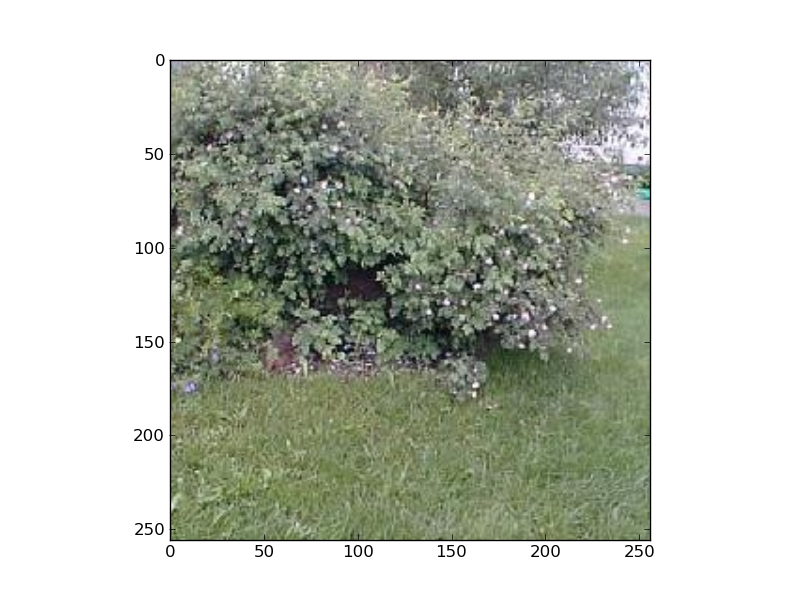
\includegraphics[width=4cm]{dbshow-2-0.png} 
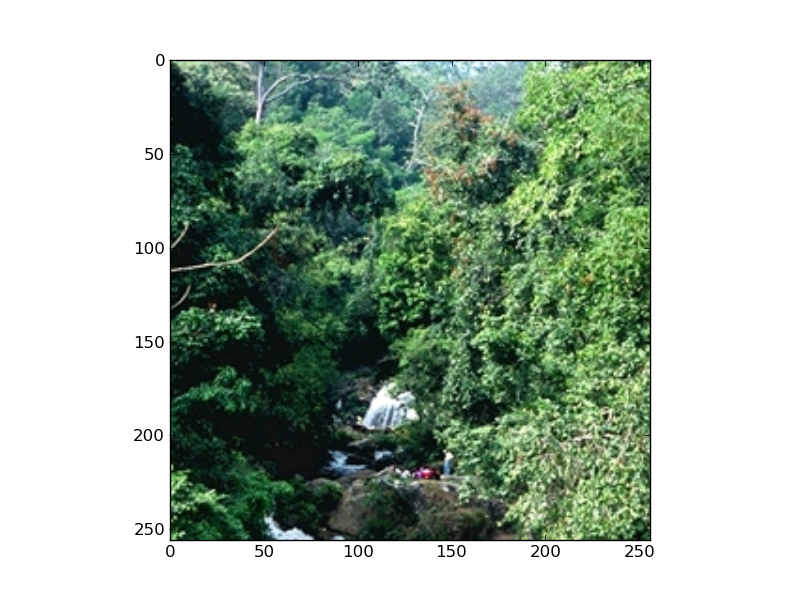
\includegraphics[width=4cm]{dbshow-2-1.png} 
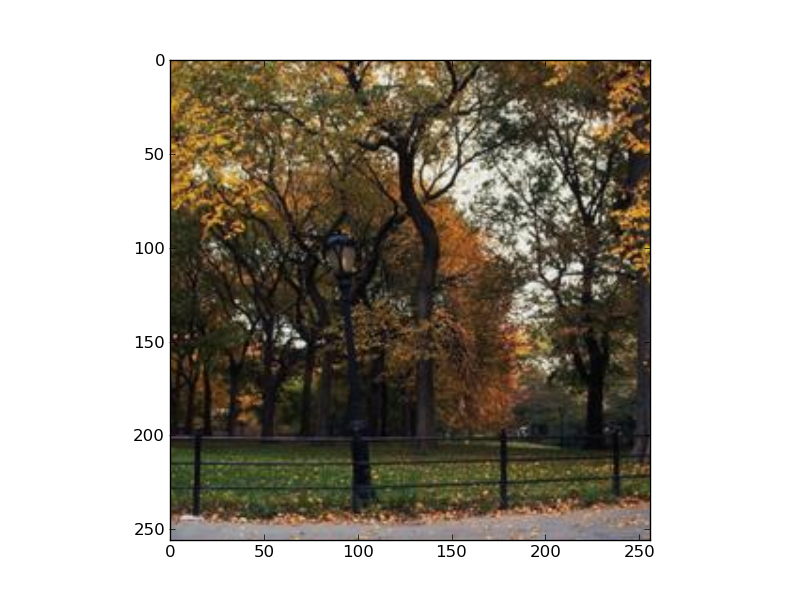
\includegraphics[width=4cm]{dbshow-2-2.png} 
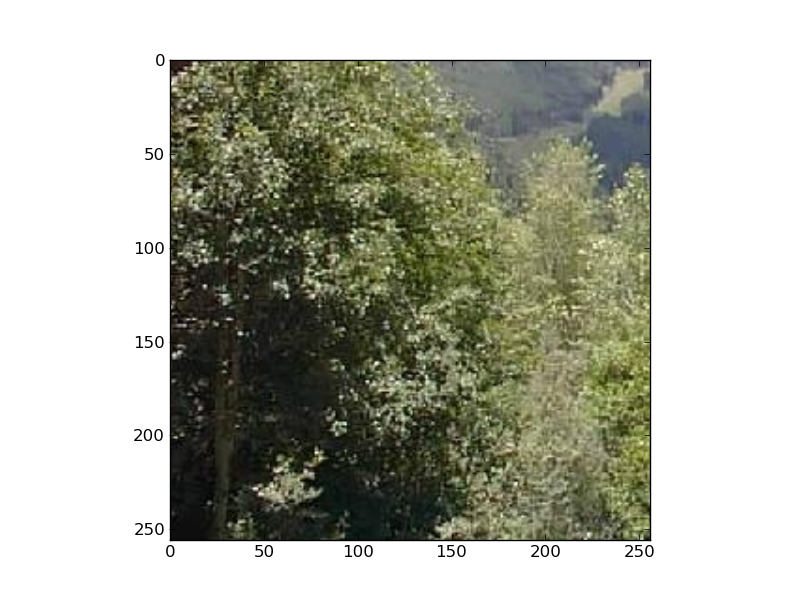
\includegraphics[width=4cm]{dbshow-2-3.png} 
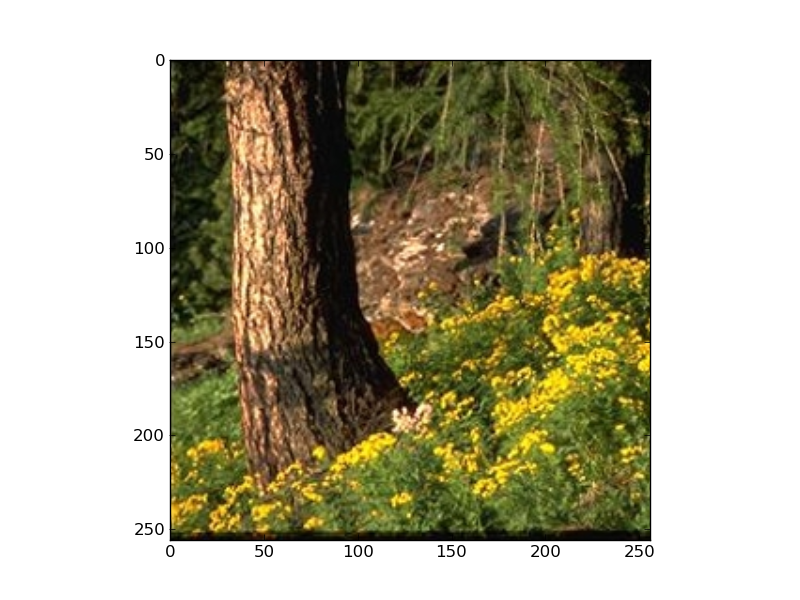
\includegraphics[width=4cm]{dbshow-2-4.png} 














\lstset{
language=bash,                % choose the language of the code
basicstyle=\footnotesize,       % the size of the fonts that are used for the code
numbers=left,                   % where to put the line-numbers
numberstyle=\footnotesize,      % the size of the fonts that are used for the line-numbers
stepnumber=5,                   % the step between two line-numbers. If it's 1 each line will be numbered
numbersep=5pt,                  % how far the line-numbers are from the code
backgroundcolor=\color{white},  % choose the background color. You must add \usepackage{color}
showspaces=false,               % show spaces adding particular underscores
showstringspaces=false,         % underline spaces within strings
showtabs=false,                 % show tabs within strings adding particular underscores
frame=single,	                % adds a frame around the code
tabsize=2,	                % sets default tabsize to 2 spaces
captionpos=b,                   % sets the caption-position to bottom
breaklines=true,                % sets automatic line breaking
breakatwhitespace=false         % sets if automatic breaks should only happen at whitespace
}
\begin{lstlisting}
python train_model.py \
    -m "#M('naive')-{'mean':L('meanvariancemodel.SimpleMeanVarianceModel')}" \
    --db "image_directory" \
    --dbargs "'path' : '/home/tranx/databases/8outdoorcategories/', 'filtere':'^$cat(.*).jpg$'" \
    -s "outdoors-$cat" 

ls /home/tranx/models/MnaivemeanLmeanvariancemodelSimpleMeanVarianceModel-image_directory-std/mean/lowlevel

\end{lstlisting}






So by running the previous command we have trained a model.
We can see that he associated datas have been stored in a file.


We know ask to train a model with each category we want to able to recognize...
Here we do simply do it by the mean of shell scripting. But we coul have used python
scripting instead to.










\lstset{
language=bash,                % choose the language of the code
basicstyle=\footnotesize,       % the size of the fonts that are used for the code
numbers=left,                   % where to put the line-numbers
numberstyle=\footnotesize,      % the size of the fonts that are used for the line-numbers
stepnumber=5,                   % the step between two line-numbers. If it's 1 each line will be numbered
numbersep=5pt,                  % how far the line-numbers are from the code
backgroundcolor=\color{white},  % choose the background color. You must add \usepackage{color}
showspaces=false,               % show spaces adding particular underscores
showstringspaces=false,         % underline spaces within strings
showtabs=false,                 % show tabs within strings adding particular underscores
frame=single,	                % adds a frame around the code
tabsize=2,	                % sets default tabsize to 2 spaces
captionpos=b,                   % sets the caption-position to bottom
breaklines=true,                % sets automatic line breaking
breakatwhitespace=false         % sets if automatic breaks should only happen at whitespace
}
\begin{lstlisting}
for cat in coast forest insidecity highway mountain opencountry street tallbuilding; do
  python train_model.pyc \
    -m "#M('naive')-{'mean':L('meanvariancemodel.SimpleMeanVarianceModel')}" \
    --db image_directory \
    --dbargs "'path' : '/home/tranx/databases/8outdoorcategories/', 'filtere':'^$cat(.*).jpg$'" \
    -s "outdoors-$cat" 
done

\end{lstlisting}







Now let's visualize what the model has learn. We have no specific program here.
We will directly load the data form our model file, and ask the computer to display it.
The first of all we can visualize the mean value for each image category.







\lstset{
language=Python,                % choose the language of the code
basicstyle=\footnotesize,       % the size of the fonts that are used for the code
numbers=left,                   % where to put the line-numbers
numberstyle=\footnotesize,      % the size of the fonts that are used for the line-numbers
stepnumber=5,                   % the step between two line-numbers. If it's 1 each line will be numbered
numbersep=5pt,                  % how far the line-numbers are from the code
backgroundcolor=\color{white},  % choose the background color. You must add \usepackage{color}
showspaces=false,               % show spaces adding particular underscores
showstringspaces=false,         % underline spaces within strings
showtabs=false,                 % show tabs within strings adding particular underscores
frame=single,	                % adds a frame around the code
tabsize=2,	                % sets default tabsize to 2 spaces
captionpos=b,                   % sets the caption-position to bottom
breaklines=true,                % sets automatic line breaking
breakatwhitespace=false         % sets if automatic breaks should only happen at whitespace
}
\begin{lstlisting}
from jfli.stats.meanvariancemodel import SimpleMeanVarianceModel as smvm
pyplot.clf()
categories=["coast","forest","insidecity","highway","mountain","opencountry","street","tallbuilding"]
pyplot.figure(figsize=(12,6))
for c in range(8):
  pyplot.subplot(240+(c+1))
  r=smvm.load(file("/home/tranx/models/MnaivemeanLmeanvariancemodelSimpleMeanVarianceModel-image_directory-outdoors-%s/mean/lowlevel"%(categories[c],))).mean()/256.
  pyplot.imshow(r)
  pyplot.title("Mean "+categories[c])

pyplot.show()

\end{lstlisting}















\noindent
\includegraphics[width=\textwidth]{pyfig-2cdc0bfe96be908b647d9223849d9e02.pdf}






Now we can also visualize the standard deviation for each image category.







\lstset{
language=Python,                % choose the language of the code
basicstyle=\footnotesize,       % the size of the fonts that are used for the code
numbers=left,                   % where to put the line-numbers
numberstyle=\footnotesize,      % the size of the fonts that are used for the line-numbers
stepnumber=5,                   % the step between two line-numbers. If it's 1 each line will be numbered
numbersep=5pt,                  % how far the line-numbers are from the code
backgroundcolor=\color{white},  % choose the background color. You must add \usepackage{color}
showspaces=false,               % show spaces adding particular underscores
showstringspaces=false,         % underline spaces within strings
showtabs=false,                 % show tabs within strings adding particular underscores
frame=single,	                % adds a frame around the code
tabsize=2,	                % sets default tabsize to 2 spaces
captionpos=b,                   % sets the caption-position to bottom
breaklines=true,                % sets automatic line breaking
breakatwhitespace=false         % sets if automatic breaks should only happen at whitespace
}
\begin{lstlisting}
from jfli.stats.meanvariancemodel import SimpleMeanVarianceModel as smvm
pyplot.clf()
categories=["coast","forest","insidecity","highway","mountain","opencountry","street","tallbuilding"]
pyplot.figure(figsize=(12,6))
for c in range(8):
  pyplot.subplot(240+(c+1))
  r=smvm.load(file("/home/tranx/models/MnaivemeanLmeanvariancemodelSimpleMeanVarianceModel-image_directory-outdoors-%s/mean/lowlevel"%(categories[c],))).std()/256.
  pyplot.imshow(r)
  pyplot.title("StdErr "+categories[c])

pyplot.show()

\end{lstlisting}















\noindent
\includegraphics[width=\textwidth]{pyfig-fee7719bf13fdfad362282fac5cd5c83.pdf}






Another way of querying a model is to sample elements from it:







\lstset{
language=Python,                % choose the language of the code
basicstyle=\footnotesize,       % the size of the fonts that are used for the code
numbers=left,                   % where to put the line-numbers
numberstyle=\footnotesize,      % the size of the fonts that are used for the line-numbers
stepnumber=5,                   % the step between two line-numbers. If it's 1 each line will be numbered
numbersep=5pt,                  % how far the line-numbers are from the code
backgroundcolor=\color{white},  % choose the background color. You must add \usepackage{color}
showspaces=false,               % show spaces adding particular underscores
showstringspaces=false,         % underline spaces within strings
showtabs=false,                 % show tabs within strings adding particular underscores
frame=single,	                % adds a frame around the code
tabsize=2,	                % sets default tabsize to 2 spaces
captionpos=b,                   % sets the caption-position to bottom
breaklines=true,                % sets automatic line breaking
breakatwhitespace=false         % sets if automatic breaks should only happen at whitespace
}
\begin{lstlisting}
import scipy,numpy
import pylab as pyplot

from jfli.stats.meanvariancemodel import SimpleMeanVarianceModel as smvm
pyplot.clf()
categories=["coast","forest","insidecity","highway","mountain","opencountry","street","tallbuilding"]
c=0
pyplot.figure(figsize=(12,3))
for sampl in range(8):
  pyplot.subplot(180+(sampl+1))
  r=smvm.load(file("/home/tranx/models/MnaivemeanLmeanvariancemodelSimpleMeanVarianceModel-image_directory-outdoors-%s/mean/lowlevel"%(categories[c],))).sample(1)[0]/256.
  pyplot.imshow(r)
  pyplot.title("Sample "+str(sampl))

pyplot.show()

\end{lstlisting}















\noindent
\includegraphics[width=\textwidth]{pyfig-3ea74af8fd3b058c1e372545ffdcbd4c.pdf}














\noindent
\includegraphics[width=\textwidth]{pyfig-5385e07d4b565b297f5da1414d78ada0.pdf}











\noindent
\includegraphics[width=\textwidth]{pyfig-90b7d75b8c28657968975bd2a79eeefc.pdf}











\noindent
\includegraphics[width=\textwidth]{pyfig-c19f6a6e8b897128ef3084884f522bbf.pdf}











\noindent
\includegraphics[width=\textwidth]{pyfig-406efa5de7b02585ee3b98bb76335ed7.pdf}











\noindent
\includegraphics[width=\textwidth]{pyfig-dbd5b1f2a900afa9cf8726b65085be08.pdf}











\noindent
\includegraphics[width=\textwidth]{pyfig-4550967043313b1e03d4219fe9c8f185.pdf}











\noindent
\includegraphics[width=\textwidth]{pyfig-9c4f68d7acb57548dcfc835e0fba3591.pdf}






Same effects could be achieved by executing the command











\lstset{
language=bash,                % choose the language of the code
basicstyle=\footnotesize,       % the size of the fonts that are used for the code
numbers=left,                   % where to put the line-numbers
numberstyle=\footnotesize,      % the size of the fonts that are used for the line-numbers
stepnumber=5,                   % the step between two line-numbers. If it's 1 each line will be numbered
numbersep=5pt,                  % how far the line-numbers are from the code
backgroundcolor=\color{white},  % choose the background color. You must add \usepackage{color}
showspaces=false,               % show spaces adding particular underscores
showstringspaces=false,         % underline spaces within strings
showtabs=false,                 % show tabs within strings adding particular underscores
frame=single,	                % adds a frame around the code
tabsize=2,	                % sets default tabsize to 2 spaces
captionpos=b,                   % sets the caption-position to bottom
breaklines=true,                % sets automatic line breaking
breakatwhitespace=false         % sets if automatic breaks should only happen at whitespace
}
\begin{lstlisting}
python sample_model.py \
    -m "#M('naive')-{'mean':L('meanvariancemodel.SimpleMeanVarianceModel')}" \
    --db "image_directory" \
    --dbargs "'path' : '/home/tranx/databases/8outdoorcategories/', 'filtere':'^$cat(.*).jpg$'" \
    -s "outdoors-$cat" 
    --model_path "//mean"
    -n 10

\end{lstlisting}








Similar stuffs may be done on other models , such as fourrier transforms of images












\lstset{
language=bash,                % choose the language of the code
basicstyle=\footnotesize,       % the size of the fonts that are used for the code
numbers=left,                   % where to put the line-numbers
numberstyle=\footnotesize,      % the size of the fonts that are used for the line-numbers
stepnumber=5,                   % the step between two line-numbers. If it's 1 each line will be numbered
numbersep=5pt,                  % how far the line-numbers are from the code
backgroundcolor=\color{white},  % choose the background color. You must add \usepackage{color}
showspaces=false,               % show spaces adding particular underscores
showstringspaces=false,         % underline spaces within strings
showtabs=false,                 % show tabs within strings adding particular underscores
frame=single,	                % adds a frame around the code
tabsize=2,	                % sets default tabsize to 2 spaces
captionpos=b,                   % sets the caption-position to bottom
breaklines=true,                % sets automatic line breaking
breakatwhitespace=false         % sets if automatic breaks should only happen at whitespace
}
\begin{lstlisting}
for cat in coast forest insidecity highway mountain opencountry street tallbuilding; do
  python train_model.py \
    -m "#M('image.gray')|{'fft':M('image.fft')-{'mean':L('meanvariancemodel.SimpleMeanVarianceModel')}}" \
    --db image_directory \
    --dbargs "'path' : '/home/tranx/databases/8outdoorcategories/', 'filtere':'^$cat(.*).jpg$'" \
    -s "outdoors-$cat" 
done

\end{lstlisting}













\lstset{
language=Python,                % choose the language of the code
basicstyle=\footnotesize,       % the size of the fonts that are used for the code
numbers=left,                   % where to put the line-numbers
numberstyle=\footnotesize,      % the size of the fonts that are used for the line-numbers
stepnumber=5,                   % the step between two line-numbers. If it's 1 each line will be numbered
numbersep=5pt,                  % how far the line-numbers are from the code
backgroundcolor=\color{white},  % choose the background color. You must add \usepackage{color}
showspaces=false,               % show spaces adding particular underscores
showstringspaces=false,         % underline spaces within strings
showtabs=false,                 % show tabs within strings adding particular underscores
frame=single,	                % adds a frame around the code
tabsize=2,	                % sets default tabsize to 2 spaces
captionpos=b,                   % sets the caption-position to bottom
breaklines=true,                % sets automatic line breaking
breakatwhitespace=false         % sets if automatic breaks should only happen at whitespace
}
\begin{lstlisting}
from jfli.stats.meanvariancemodel import SimpleMeanVarianceModel as smvm
pyplot.clf()
categories=["coast","forest","insidecity","highway","mountain","opencountry","street","tallbuilding"]
pyplot.figure(figsize=(12,6))
for c in range(8):
  pyplot.subplot(240+(c+1))
  r=smvm.load(file("/home/tranx/models/MimagegrayfftMimagefftmeanLmeanvariancemodelSimpleMeanVarianceModel-image_directory-outdoors-%s/fft/mean/lowlevel"%(categories[c],))).mean()
  r=numpy.roll(numpy.roll(numpy.log(numpy.abs(r)).squeeze(),r.shape[0]//2,axis=0),r.shape[0]//2,axis=1)
  pyplot.imshow(r,vmin=0,vmax=16)
  pyplot.title("Mean FFT of "+categories[c])
  pyplot.colorbar()

pyplot.show()

\end{lstlisting}















\noindent
\includegraphics[width=\textwidth]{pyfig-8003959c06a2a3e6c93397cbd29c953d.pdf}










\lstset{
language=Python,                % choose the language of the code
basicstyle=\footnotesize,       % the size of the fonts that are used for the code
numbers=left,                   % where to put the line-numbers
numberstyle=\footnotesize,      % the size of the fonts that are used for the line-numbers
stepnumber=5,                   % the step between two line-numbers. If it's 1 each line will be numbered
numbersep=5pt,                  % how far the line-numbers are from the code
backgroundcolor=\color{white},  % choose the background color. You must add \usepackage{color}
showspaces=false,               % show spaces adding particular underscores
showstringspaces=false,         % underline spaces within strings
showtabs=false,                 % show tabs within strings adding particular underscores
frame=single,	                % adds a frame around the code
tabsize=2,	                % sets default tabsize to 2 spaces
captionpos=b,                   % sets the caption-position to bottom
breaklines=true,                % sets automatic line breaking
breakatwhitespace=false         % sets if automatic breaks should only happen at whitespace
}
\begin{lstlisting}
import scipy.ndimage
from jfli.stats.meanvariancemodel import SimpleMeanVarianceModel as smvm
pyplot.clf()
categories=["coast","forest","insidecity","highway","mountain","opencountry","street","tallbuilding"]
pyplot.figure(figsize=(12,6))
for c in range(8):
  pyplot.subplot(240+(c+1))
  r=smvm.load(file("/home/tranx/models/MimagegrayfftMimagefftmeanLmeanvariancemodelSimpleMeanVarianceModel-image_directory-outdoors-%s/fft/mean/lowlevel"%(categories[c],))).mean()
  r=numpy.roll(numpy.roll(numpy.log(numpy.abs(r)).squeeze(),r.shape[0]//2,axis=0),r.shape[0]//2,axis=1)
  Z =scipy.ndimage.gaussian_filter(r,10)
  pyplot.contour(Z,numpy.arange(2.,14**.5,0.2)**2)
  pyplot.title("Mean FFT of "+categories[c])
  pyplot.colorbar()

pyplot.show()

\end{lstlisting}















\noindent
\includegraphics[width=\textwidth]{pyfig-e15cf9d59ecdc15b92bb756c893f4341.pdf}













\lstset{
language=Python,                % choose the language of the code
basicstyle=\footnotesize,       % the size of the fonts that are used for the code
numbers=left,                   % where to put the line-numbers
numberstyle=\footnotesize,      % the size of the fonts that are used for the line-numbers
stepnumber=5,                   % the step between two line-numbers. If it's 1 each line will be numbered
numbersep=5pt,                  % how far the line-numbers are from the code
backgroundcolor=\color{white},  % choose the background color. You must add \usepackage{color}
showspaces=false,               % show spaces adding particular underscores
showstringspaces=false,         % underline spaces within strings
showtabs=false,                 % show tabs within strings adding particular underscores
frame=single,	                % adds a frame around the code
tabsize=2,	                % sets default tabsize to 2 spaces
captionpos=b,                   % sets the caption-position to bottom
breaklines=true,                % sets automatic line breaking
breakatwhitespace=false         % sets if automatic breaks should only happen at whitespace
}
\begin{lstlisting}
from jfli.stats.meanvariancemodel import SimpleMeanVarianceModel as smvm
from jfli.graphics.rescale import Rescaler2d
from matplotlib import cm
from mpl_toolkits.mplot3d import Axes3D

categories=["coast","forest","insidecity","highway","mountain","opencountry","street","tallbuilding"]
f=pyplot.figure(figsize=(6,6))
c=0
ax = Axes3D(f)
r=smvm.load(file("/home/tranx/models/MimagegrayfftMimagefftmeanLmeanvariancemodelSimpleMeanVarianceModel-image_directory-outdoors-%s/fft/mean/lowlevel"%(categories[c],))).mean()
r=numpy.roll(numpy.roll(numpy.log(numpy.abs(r)).squeeze(),r.shape[0]//2,axis=0),r.shape[0]//2,axis=1).squeeze()
X = numpy.arange(0, r.shape[1], 4)
Y = numpy.arange(0, r.shape[0], 4)
X, Y = numpy.meshgrid(X, Y)
Z =Rescaler2d((r.shape[0]//4, r.shape[1]//4)).process(r)
ax.plot_surface(X, Y, Z, rstride=1, cstride=1, cmap=cm.hot)

\end{lstlisting}











\noindent \includegraphics[width=4cm]{pyfig-6dcb223af46511fdca88084565f0a06f.pdf}            \noindent \includegraphics[width=4cm]{pyfig-6d984e99a9cb8c992cfe5955f6c697f4.pdf}            \noindent \includegraphics[width=4cm]{pyfig-90d2717e13d07118323942f8dfdf273c.pdf}            \noindent \includegraphics[width=4cm]{pyfig-735c7d482722834e4b54679b5542dcad.pdf}             \noindent \includegraphics[width=4cm]{pyfig-2be4eb4fbb56289fb72ab837f5f1de70.pdf}            \noindent \includegraphics[width=4cm]{pyfig-be46ce80af5bcaefdb7a38447be23d59.pdf}            \noindent \includegraphics[width=4cm]{pyfig-b065e7a97d586af83f8bbd3249781afa.pdf}            \noindent \includegraphics[width=4cm]{pyfig-be4d96c4e90874687e197b3405bba8fb.pdf} 









\section{Saving and Reading Track Files}
Dynamic Datastreams are great for prototyping. But sometimes they are too slow for what we need.
Or sometime we may desire to save some datas to reexploit them later in different.

These are the goal of trackfiles.

Trackfiles are designed to be seeked efficiently, and to support very large amount of datas.


TODO






\section{Improving / Repairement}
One of the thing that structures allow us is to instantiate new datas, and to iterate 
over space, and neighborhoods without knowning all the details.
Althougth keeping this element as python implementation, may lead to relatively slow algorithm.
This is very userful for prototyping applications.


Here is a sample application that uses an index to reconstruct an object.





\lstset{
language=Python,                % choose the language of the code
basicstyle=\footnotesize,       % the size of the fonts that are used for the code
numbers=left,                   % where to put the line-numbers
numberstyle=\footnotesize,      % the size of the fonts that are used for the line-numbers
stepnumber=5,                   % the step between two line-numbers. If it's 1 each line will be numbered
numbersep=5pt,                  % how far the line-numbers are from the code
backgroundcolor=\color{white},  % choose the background color. You must add \usepackage{color}
showspaces=false,               % show spaces adding particular underscores
showstringspaces=false,         % underline spaces within strings
showtabs=false,                 % show tabs within strings adding particular underscores
frame=single,	                % adds a frame around the code
tabsize=2,	                % sets default tabsize to 2 spaces
captionpos=b,                   % sets the caption-position to bottom
breaklines=true,                % sets automatic line breaking
breakatwhitespace=false         % sets if automatic breaks should only happen at whitespace
}
\begin{lstlisting}
class MyApp:
  def process():
      ## 1 basically decompose and create index based on elements of database1

      ## 2 decompose and query index on elements of database1, then recompose... (This should be appliable for instance to recompose a movie...)


MyApp.run()

\end{lstlisting}







\section{Multiple Tests and Recognition}
Once we've runned, one test it of course temptative to know what is globally happening.
And to make in-depth analysis of your models results.



Let's start has usual with basics :
We will just write a very very basic SVM.





\lstset{
language=Python,                % choose the language of the code
basicstyle=\footnotesize,       % the size of the fonts that are used for the code
numbers=left,                   % where to put the line-numbers
numberstyle=\footnotesize,      % the size of the fonts that are used for the line-numbers
stepnumber=5,                   % the step between two line-numbers. If it's 1 each line will be numbered
numbersep=5pt,                  % how far the line-numbers are from the code
backgroundcolor=\color{white},  % choose the background color. You must add \usepackage{color}
showspaces=false,               % show spaces adding particular underscores
showstringspaces=false,         % underline spaces within strings
showtabs=false,                 % show tabs within strings adding particular underscores
frame=single,	                % adds a frame around the code
tabsize=2,	                % sets default tabsize to 2 spaces
captionpos=b,                   % sets the caption-position to bottom
breaklines=true,                % sets automatic line breaking
breakatwhitespace=false         % sets if automatic breaks should only happen at whitespace
}
\begin{lstlisting}
python simple_svm_train_and_test.py --db labeled_databases_from_labels --dbargs "'labels':['dalmatian','ant','starfish']"   

\end{lstlisting}











\begin{verbatim}
Training svm nr.0                                                                                                                                                                                           
60                                                                                                                                                                                                           
Done.                                                                                                                                                                                                        
Training svm nr.1                                                                                                                                                                                           
60                                                                                                                                                                                                           
Done.                                                                                                                                                                                                        
Training svm nr.2                                                                                                                                                                                           
60                                                                                                                                                                                                           
Done.                                                                                                                                                                                                        
Testing svm nr. 0                                                                                                                                                                                            
ant 81.6666666667 %                                                                                                                                                                                          
Testing svm nr. 1                                                                                                                                                                                            
dalmatian 73.3333333333 %                                                                                                                                                                                    
Testing svm nr. 2                                                                                                                                                                                            
starfish 76.6666666667 %     
\end{verbatim}

Althougth simple_svm_train_and_test.py is not very interesting because it does not allow you to save the data. It is maybe a good way
to a priori test model.



The other thing that you are likely to want to do is to know out of differents models, which model is explaining the best your datas.


We will do Object Classification on Caltech 101.
With a traditional model






\lstset{
language=Python,                % choose the language of the code
basicstyle=\footnotesize,       % the size of the fonts that are used for the code
numbers=left,                   % where to put the line-numbers
numberstyle=\footnotesize,      % the size of the fonts that are used for the line-numbers
stepnumber=5,                   % the step between two line-numbers. If it's 1 each line will be numbered
numbersep=5pt,                  % how far the line-numbers are from the code
backgroundcolor=\color{white},  % choose the background color. You must add \usepackage{color}
showspaces=false,               % show spaces adding particular underscores
showstringspaces=false,         % underline spaces within strings
showtabs=false,                 % show tabs within strings adding particular underscores
frame=single,	                % adds a frame around the code
tabsize=2,	                % sets default tabsize to 2 spaces
captionpos=b,                   % sets the caption-position to bottom
breaklines=true,                % sets automatic line breaking
breakatwhitespace=false         % sets if automatic breaks should only happen at whitespace
}
\begin{lstlisting}
class MyModel(genericmodel.GenericModel):
   def __init__(self):
       pass
   def compute():
       res=pysift.sift(x)
   def init_featurefilter():
        pass

\end{lstlisting}


























\subsection{Filtering Adult Material}
\subsubsection{Filtering Adult Material based on Skin colors}







\subsubsection{Filtering Adult Material based on Skin Texture}






\subsection{Classifying Natural Scenes}









!!!Not yet finished!!!

\end{document}
